\documentclass[a4paper,14pt,russian,utf8,nocolumnsxix,nocolumnxxxi,nocolumnxxxii]{eskdtext}
\usepackage{diplom} 

 
\begin{document}
%\renewcommand*\contentsname{ОГЛАВЛЕНИЕ}
\tableofcontents %ОГЛАВЛЕНИЕ

\pagebreak

\section*{ВВЕДЕНИЕ}
\addcontentsline{toc}{section}{ВВЕДЕНИЕ}
В настоящее время, с развитием компьютерных технологий, использование систем автоматического распознавания речи в качестве интерфейса приобретает все большую популярность. Однако, создание таких систем является нетривиальной задачей.

Проблеме распознавания речевых образов посвящено большое количество работ различных авторов.\cite{mazurenko,vincuk,spokenlang} Успешное решение данной проблемы позволит осуществить частичную замену интеллектуальной деятельности человека действием автоматов. Выбор принципа распознавания речевых сигналов зависит от типа системы, объема словаря, требований к скорости и качеству работы системы. 

В случае реализации технологии распознавания с малым словарем (до 50 слов) применяют алгоритмы сравнения введенного образца с существующими в базе эталонами. При этом необходимо выбрать критерии сравнения, а также функцию принятия решения. В качестве критерия сравнения выступают характеристики речевого сигнала, которые несут основную информацию о его особенностях. Технологии распознавания слитной речи используют алгоритмы на основе скрытых моделей Маркова или обучаемых нейронных сетей.

В данной работе выполнен обзор нескольких различных подходов к решению проблемы распознавания устной речи, а также реализован и исследован алгоритм динамического трансформирования времени (DTW), применяемый в системах с ограниченным словарем

Применение алгоритма динамического трансформирования времени связано с тем, что каждая реализация произнесенного слова может отличаться от любой другой по целому ряду признаков. Например, по частоте или громкости. Также анализируемый речевой сигнал может быть растянут или сжат по времени относительно образца, с которым производится сравнение. 

Алгоритм динамического трансформирования времени (DTW) вычисляет оптимальную последовательность трансформации (деформации) времени между двумя временными рядами. Алгоритм вычисляет значения деформации между двумя рядами и расстояние между ними.\cite{sakoe}

Также в ходе выполнения работы был исследован способ представления речевого сигнала в виде мел-частотных кепстральных коэффициентов (MFCC). В соответствии с теорией речеобразования \cite{agran,rabiner1,sorokin} речь представляет собой акустическую волну, которая излучается системой органов: легкими, бронхами и трахеей, а затем преобразуется в голосовом тракте. Если предположить, что источники возбуждения и форма голосового тракта относительно независимы, речевой аппарат человека можно представить в виде совокупности генераторов тоновых сигналов и шумов, а также фильтров. Использование кепстрального анализа позволяет развернуть речевой сигнал, и получить информацию о состоянии артикуляционного аппарата, которая недоступна в частотной или временной области. Выбор такого способа описания сигнала был сделан на основании работы \cite{davis}, в которой показано, что представление спектра сигнала в виде мел-частотных коэффициентов может успешно применяться в распознавании речи.

Целью работы является разработка и исследование алгоритма распознавания речи, основанного на анализе мел-частотных кепстральных коэффициентов.

Для достижения поставленной цели требуется решить следующие задачи:
\begin{enumerate}[1)]
	\item Провести анализ моделей речевого сигнала;
	\item Изучить подходы к решению задачи распознавания устной речи;
	\item Реализовать алгоритм получения описания речевого сигнала и решающую функцию;
	\item Исследовать реализованный алгоритм.
\end{enumerate}

\pagebreak

\section{Модели речевых сигналов}
%\addcounter{section}{1}
%\addcontentsline{toc}{section}{Модели речевых сигналов}
\subsection {Теория речеобразования}
\begin{figure}[ht]
	\centering
	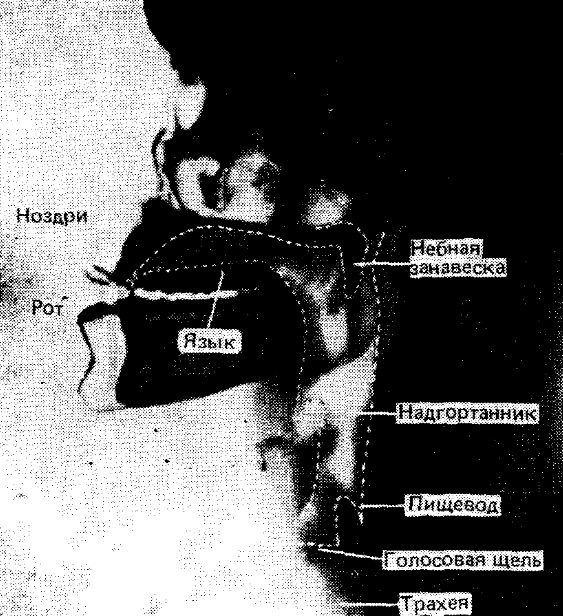
\includegraphics[width=120mm]{xray.jpg}			
	\caption{Рентгеновский снимок речеобразующих органов человека}
	\label{xray}
\end{figure}
На рентгеновском снимке (рисунок \ref{xray}) показаны наиболее важные органы речеобразующей системы человека. Голосовой тракт, который на рисунке обведен пунктиром, начинается с прохода между голосовыми связками, называемого голосовой щелью, и заканчивается у губ. Голосовой тракт, таком образом, состоит из гортани (от пищевода до рта) и рта, или ротовой полости. У взрослого человека общая длина голосового тракта составляет примерно 17 см. Площадь поперечного сечения голосового тракта, которая определяется положением языка, губ, челюстей и небной занавески, может изменяться от нуля до примерно 20 см\textsuperscript{2}. Носовая полость начинается у небной занавески и заканчивается ноздрями. При опущенной небной занавеске носовая полость акустически соединена с голосовым трактом и участвует в образовании носовых звуков речи. При изучении процесса речеобразования полезно изображать основные органы физической системы в таком виде, при котором становится ясной математическая сторона вопроса.

На рисунке \ref{trakt} показано подробное схематическое изображение речеобразующей системы. Для полноты в диаграмму включены и такие органы, как легкие, бронхи, и трахея, расположенные ниже гортани. Совокупность этих органов служит источником энергии для образования речи.\cite{rabiner1} 
\begin{figure}[ht]	
	\centering
	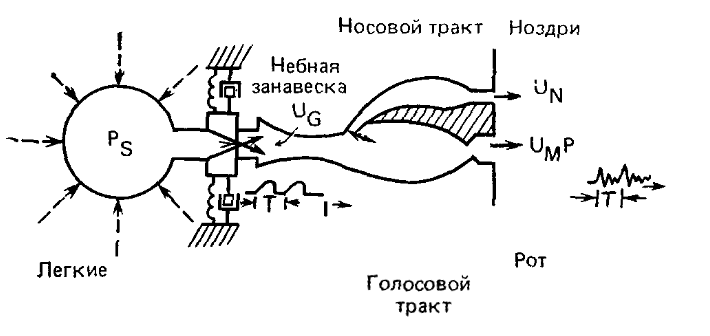
\includegraphics[width=120mm]{trakt.png}			
	\caption{Схематическое изображение речеобразующих органов человека}
	\label{trakt}
\end{figure}

Речь представляет собой акустическую волну, которая вначале излучается этой системой при выталкивании воздуха из легких и затем преобразуется в голосовом тракте. В качестве примера на рисунке \ref{shpaga_graph} показано речевое колебание, соответствующее слову <<шпага>>, произнесенному мужским голосом. Основные особенности колебания легко объяснить на основе подробного анализа механизма образования речи.

\begin{figure}[H]	
	\centering
	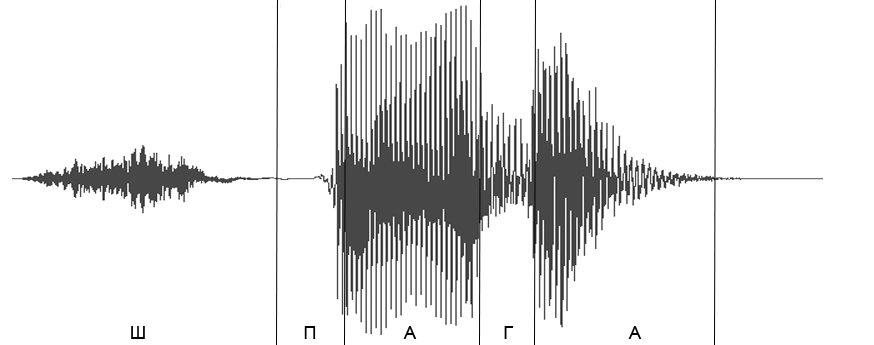
\includegraphics[width=120mm]{shpaga_graph.png}			
	\caption{Речевое колебание, соответствующее слову <<шпага>>}
	\label{shpaga_graph}
\end{figure}
Звуки речи могут быть разделены на три четко выраженные группы по типу возбуждения.
\begin{itemize}

\item Вокализованные звуки (например, звук <<А>>, предсталенный на рисунке \ref{shpaga_graph}) образуются проталкиванием воздуха через голосовую щель, при котором периодически напрягаются и расслабляются голосовые связки и возникает квазипериодическая последовательность импульсов потока воздуха, возбуждающая голосовой тракт.
\item Фрикативные или невокализованные звуки (звук <<Ш>> на рисунке \ref{shpaga_graph}) генерируются при сужении голосового тракта в каком-либо месте (обычно в конце рта) и проталкивании воздуха через суженное место со скоростью, достаточно высокой для образования турбулентного воздушного потока. Таким образом, формируется источник широкополосного шума, возбуждающего голосовой тракт. 
\item Взрывные звуки (звук <<П>> на рисунке \ref{shpaga_graph}) характеризуются тем, что при их произнесении голосовой тракт полностью закрывается. За этой смычкой возникает сильное сжатие воздуха. Затем воздух резко\\ высвобождается.\cite{rabiner1}
\end{itemize}


\begin{figure}[H]	
	\centering
	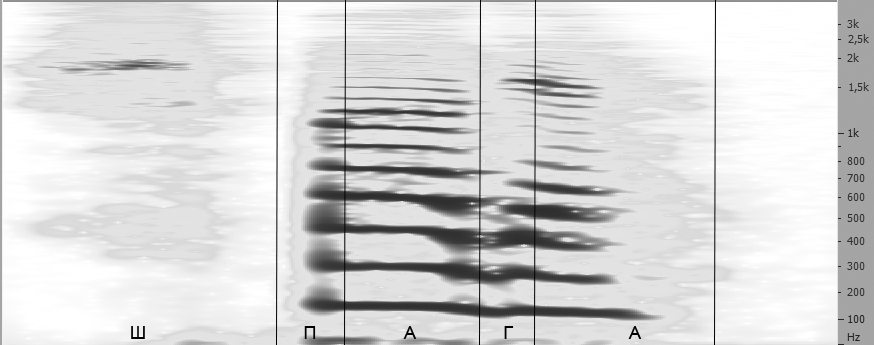
\includegraphics[width=120mm]{shpaga_spect.png}			
	\caption{Спектрограмма, соответствующая слову <<шпага>>}
	\label{shpaga_spect}
\end{figure}
Голосовой тракт и носовая полость показаны на рисунке \ref{trakt} в виде труб с переменной по продольной оси площадью поперечного сечения. При прохождении звуовых волн через эти трубы их частотный спектр изменяется в соответствии с частотной избирательностью трубы. Этот эффект похож на резонансные явления, происходящие в трубах органов и духовых музыкальных инструментов. При описании речеобразования резонансные частоты трубы голосового тракта называют формантными частотами или просто формантами. Формантные частоты зависят от конфигурации и размеров голосового тракта: произвольная форма тракта может быть описана набором формантных частот. Различные звуки образуются путем изменения формы голосового тракта. Переменные во времени спектральные характеристики речевого сигнала могут быть представлены в виде спектрограммы, на которой по вертикальной оси отложена частота, а по горизонтальной --- время. Спектрограмма произнесенного слова <<шпага>> показана на рисунке \ref{shpaga_spect}. Плотность зачернения графика пропорциональна энергии сигнала. Таким образом, резонансные частоты голосового тракта имеют вид затемненных областей на спектрограмме. 

\subsection{Спектральные характеристики речевых сигналов}
Фундаментальным отличием вокализованных звуков является наличие квазипериодической составляющей, которую называют основным тоном. Наличие основного тона связано с особенностями речевого аппарата человека. Находящиеся в начале голосового тракта голосовые связки (рисунок \ref{larynx}) периодически перекрывают воздушный поток с определенной частотой. Различие в тембрах разных звуков обусловлено изменением формы голосового тракта.\cite{rabiner_eng}
\begin{figure}[H]	
	\centering
	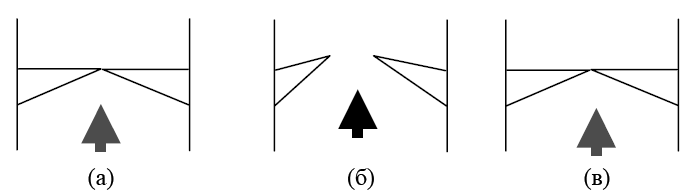
\includegraphics[width=120mm]{larynx.png}			
	\caption{Цикл сокращения голосовых связок. (а) Связки перекрывают голосовую щель, нарастание давления; (б) Связки открываются под давлением; (в) Выравнивание давления и эластичность тканей вызывают закрытие связок.}
	\label{larynx}
\end{figure}

Голосовые связки вибрируют с различной частотой у разных людей, от 60 Гц для низкого мужского голоса до 300 Гц для высокого женского или детского голоса. Данная частота называется частотой основного тона, так как она определяет основную гармоническую составляющую речевого звука. Голосовой тракт по сути является резонатором, выделяющим более высокие гармоники основной частоты. Воспринимаемая высота звука в большей степени определяется частотой основного тона.

\begin{figure}[H]	
	\centering
	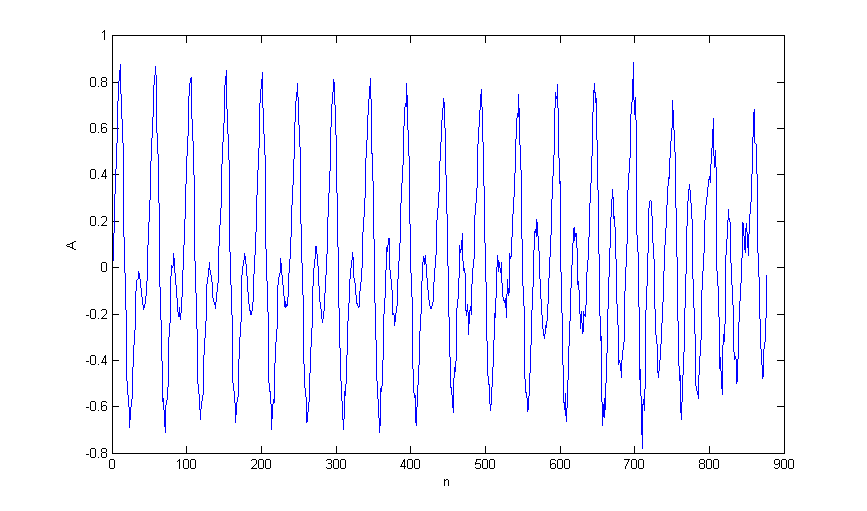
\includegraphics[width=120mm]{i1_form.png}			
	\caption{Речевое колебание, соответствующее звуку <<И>>}
	\label{i1_form}
\end{figure}

Звук <<И>>, изображенный на рисунке \ref{i1_form}, имеет спектр, показанный на рисунке \ref{i1_spect}. Форма спектра показывает неравномерное распределение энергии речевого сигнала в частотной области. Частоты, на которых сконцентрирована энергия сигнала называются формантными частотами или формантами.
\begin{figure}[H]	
	\centering
	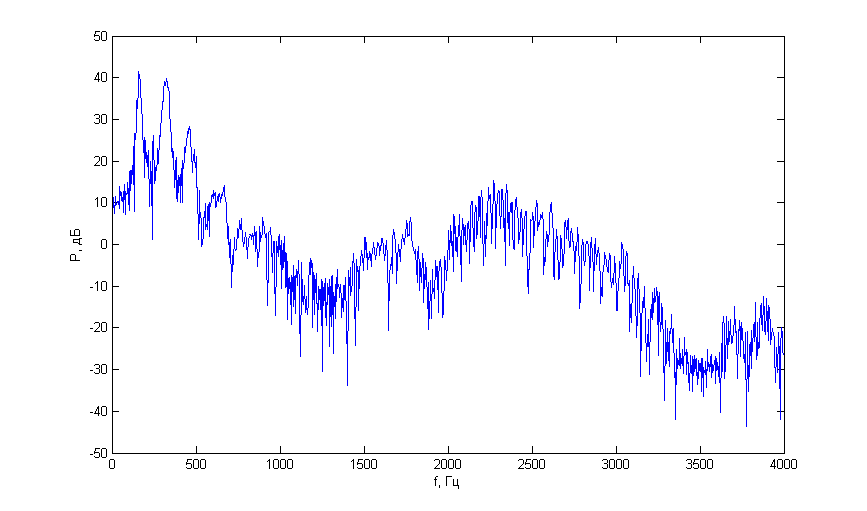
\includegraphics[width=120mm]{i1_spect.png}			
	\caption{Спектр звука <<И>>}
	\label{i1_spect}
\end{figure}

Термин форманта обозначает определенную частотную область, в которой вследствие резонанса усиливается некоторое число гармоник тона, производимого голосовыми связками, то есть в спектре звука форманта является достаточно отчетливо выделяющейся областью усиленных частот, определяемой по усредненной частотной величине. Фактически феномен форманты есть проявление работы активного полосового фильтра в составе речевого тракта. Принятое обозначение форманты --- F. Считается, что для характеристики звуков речи достаточно выделения четырех формант --- FI, FII, FIII, FIV, которые нумеруются в порядке возрастания их частоты: самая низкая форманта, ближе всех расположенная к частоте голосового источника, --- FI, за ней --- FII и т. д. Для разных звуков речи характерны определенные частотные диапазоны формант. Среднее расстояние между формантами для мужских голосов составляет приблизительно 1000 Гц, для женских и детских --- несколько больше.\cite{bondarko}

Количество формант сопоставимо с количеством резонансных полостей в речевом тракте. Каждая из формант определяется всеми участками речевого тракта, хотя степень влияния в каждом конкретном случае неодинакова. В большинстве случаев для различения гласных звуков достаточно первых двух формант, однако практически всегда количество формант в спектре звука больше двух, что указывает на более сложные связи между артикуляцией и акустическими характеристиками звука, чем при условии рассмотрения только двух первых формант.

\subsection{Кепстральные характеристики речевых сигналов}
Основой кепстрального анализа речевых сигналов является предположение, что речевой сигнал трактуется как сигнал на выходе линейной системы с медленно изменяющимися параметрами. Это предположение позволяет считать, что на коротких сегментах речевой сигнал можно рассматривать как сигнал на выходе линейной системы с постоянными параметрами, возбуждаемой либо последовательностью импульсов, либо случайным шумом. Проблема анализа сигнала сводится к измерению параметров модели и оценке изменения этих параметров с течением времени. Поскольку сигнал возбуждения и импульсная характеристика фильтра взаимодействуют через операцию свертки, задача анализа речи может рассматриваться как задача разделения компонент, участвующих в операции свертки. Такая задача иногда называется задачей обратной свертки.\cite{rabiner1} Одним из методов решения данной задачи является кепстральный анализ.
\begin{figure}[H]	
	\centering
	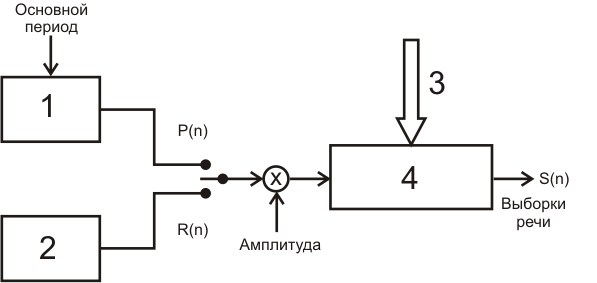
\includegraphics[width=120mm]{speech_filt.png}			
	\caption[Модель речевого аппарата в виде линейной системы]{Модель речевого аппарата в виде линейной системы
	\begin{inparaenum}[1)]
	\item
	Генератор импульсной последовательности;
	\item
	Генератор случайных чисел;
	\item
	Коэффициенты цифрового фильтра (параметры голосового тракта);
	\item
	Нестационарный цифровой фильтр.
	\end{inparaenum}}
	\label{speech_filt}
\end{figure}

Если предположить, что источники возбуждения и форма голосового тракта относительно независимы, речевой аппарат человека возможно представить в виде совокупности генераторов тоновых сигналов и шумов, а также фильтров. Схема такой модели представлена на рисунке \ref{speech_filt}.

Рассматриваемые фильтры имеют постоянные характеристики на временном интервале порядка 10 мс. Поэтому на каждом интервале фильтр можно характеризовать импульсной или частотной характеристикой или набором коэффициентов, если импульсная характеристика фильтра бесконечна. Такая модель позволяет применить для анализа речевых сигналов гомоморфную развертку.


Например, задан сигнал $s_{\text{вых}}(t)$ на выходе фильтра. Требуется определить некоторую информацию о входном сигнале $s_{\text{вх}}(t)$ и самом фильтре, например, о его импульсной характеристике $h(t)$.

Выходной сигнал определяется сверткой $s_{\text{вых}}(t)=s_{\text{вх}}(t)\otimes h(t)$.

Т.к. $S_{\text{вых}}(\omega)=S_{\text{вх}}(\omega)H(\omega)$ в частотной области, то прологарифмировав получаем выражение 
\begin{equation}
ln[S^2_{\text{вых}}(\omega)]=ln[S^{2}_{\text{вх}}(\omega)]+ln[H^{2}(\omega)].
\end{equation}

Применив к нему обратное преобразование Фурье, можно получить выражение вида:

\begin{equation}
C(q)=C_{s}(q)+C_{h}(q)
\end{equation}
из которого методами линейной фильтрации может быть возможно выделить некоторые характеристики $s_{\text{вх}}(t)$ и $h(t)$.

Также $C(q)$ может быть записано в виде:
\begin{equation}
 C(q)={\frac{1}{2\pi}}\int\limits_{-\infty}^{\infty} \ln [S(\omega)]^2 e^{i\omega q}\, d\omega .
\end{equation}

Данное преобразование получило название <<кепстр>>. Аргумент q имеет размерность времени, но это особое, кепстральное время, поскольку $C(q)$ в любой момент q зависит от функции $s(t)$ исходного сигнала со спектром $S(\omega)$ заданной при $-\infty<t<\infty$. Иногда q называют «сачтота» или «кьюфренси» (анаграммы от русского <<частота>> или английского <<frequency>>).

Так как рассматриваемые в данной работе системы распознавания речи работают с дискретным представлением речевого сигнала, целесообразно привести запись кепстра в дискретной форме:
\begin{equation}
C(n)=\frac{1}{N}\sum_{k=0}^{N-1}{\ln|{X(k)}|^2e^{i\frac{2\pi}{N}kn}}, \; 0\leq n\leq N-1.
\end{equation}

Применение кепстральных характеристик как способа описания речевых сигналов рассмотрено в практической части данной работы.

\subsection{Способы описания речевых сигналов}

При распознавании речевых сигналов, как правило, оперируют не с исходным речевым сигналом, получаемым на выходе микрофона, а с так называемым описанием речевого сигнала, экономно представляющим речевой сигнал и содержащим информацию о том, что говорится. 
Обычно принято описывать (задавать) речевой сигнал последовательностью $X_{I}=\{x_{1},x_{2},\dots,x_{i},\dots,x_{I}\}$ из элементов $x_{i}$, которые являются отсчетами векторной функции $x(t)$ в дискретные равноотстоящие моменты времени $t_{i}=i\Delta T$ с шагом $\Delta T$, принимаемым равным, например, 15 мс. Тогда $I$ это длина речевого сигнала в дискретном равномерном времени с шагом $\Delta T$. Вообще говоря, может быть использовано и неравномерное время с изменяющимся шагом $\Delta T$, выбираемым, например, из диапазона 8-25 мс. В любом случае, однако, речевой сигнал будет представляться последовательностью $X_{I}$, из элементов $x_{i}$. 
Последовательности $X_{I}$ получают в результате предварительной обработки речевого сигнала на выходе микрофона, чем существенно сокращается объем информации. Так, исходный речевой сигнал, который характеризуется объемом 200000 бит/с, как правило, описывается существенно меньшим объемом информации --- от 9600 до 600 и менее бит/с, однако все еще сохраняющим существенную информацию о том, что говорится, чтобы по ней отвечать на вопросы о распознаваемом классе. 
Вопросам предварительной обработки речевого сигнала посвящено oгpoмнoe количество работ.\cite{agran,rabiner1,rabiner_eng,vincuk} Несмотря на многочисленность предложений все они сводятся к тому, что элементы речи описываются величинами, представляющими в той или иной форме мгновенные передаточную характеристику речевого тракта и параметры источников eгo возбуждения. Поскольку эти величины изменяют свои значения сравнительно медленно в процессе произнесения речи, то для подробного описания речевых сигналов вполне достаточно ограничиться временной дискретизацией элементов с шагом $\Delta T=$ 15 мс. 
Чаще Bceгo элементами речи $x_{i}$ выступают мгновенный амплитудный спектр речи или мгновенная автокорреляционная функция, мгновенный продольный профиль акустической трубы речевого тракта, мгновенные значения параметров линейной системы, представляющей речевой тракт, мгновенные значения системы двоичных признаков, характеризующих звуки по месту и способу образования и т. п. Для многих описаний речевого сигнала могут быть указаны взаимнооднозначные преобразования, позволяющие переходить от одного описания к другому. 
Элементы $x_{i}$ могут содержать компоненты, описываемые разнородными физическими величинами. Например, наряду с компонентами, представляющими форму амплитудного спектра речи или передаточную характеристику речевого тракта, могут быть компоненты, характеризующие интенсивность элемента, способ eгo образования (с участием голоса или только шума), относительную частоту основного тона и т. п. 
Последовательности $X_{I}$, элементов $x_{i}$ получают, анализируя речевой сигнал на интервале (окне) анализа продолжительностью $\Delta T'\geq \Delta T$ и перемещая это окно вдоль оси времени с шагом $\Delta T$. Таким образом, интервалы анализа либо соприкасаются, либо перекрываются.\cite{vincuk}
\pagebreak

\section [Обзор методов и алгоритмов распознавания речи]{Обзор методов и алгоритмов\\ распознавания речи}
\setcounter{figure}{0} 

\subsection{Общие принципы систем распознавания речи}
Теория распознавания образов --- раздел кибернетики, развивающий теоретические основы и методы классификации и идентификации предметов, явлений, процессов, сигналов, ситуаций и обйъектов, которые характеризуются конечным набором некоторых свойств и признаков.

Создание искусственных систем распознавания образов остается сложной теоретической и технической проблемой. Необходимость в таком распознавании возникает в самых разных областях --- от военного дела и систем безопасности до оцифровки всевозможных аналоговых сигналов. Традиционно задачи распознавания образов включают в круг задач искусственного интеллекта.

В распознавании образов можно выделить два основных направления\cite{gorelik}:
\begin{itemize}
\item
Изучение способностей к распознаванию, которыми обладают живые существа, объяснение и моделирование их;
\item
Развитие теории и методов построения устройств, предназначенных для решения отдельных задач в прикладных целях.
\end{itemize}

Распознавание речи как частный случай распознавания образов включает в себя ряд подзадач: шумоочистка,  первичная обработка, акустико-фонетическое преобразование, обеспечение независимости от диктора. Шумоочистка позволяет повысить отношение сигнал/шум. Первичная обработка формирует из исходного речевого сигнала последовательность векторов параметров.  Акустико-фонетичес\-кое преобразование ставит в соответствие текущему вектору параметров гипотезу о его фонетической природе. Языковые модели верхних уровней позволяют из множества гипотез, порождённых на акустико-фонетическом уровне, выделить корректные.

Современные системы распознавания речи по применяемым методам могут быть разделены на четыре больших класса:
\begin{itemize}
\item
Методы дискриминатного анализа, основанные на Байесовской дискриминации;
\item
Скрытые модели Маркова;
\item
Динамическое программирование;
\item
Нейронные сети.
\end{itemize}

\subsection{Дискриминантный анализ}
Дискриминантный анализ является разделом многомерного статистического анализа, который позволяет изучать различия между двумя и более группами объектов по нескольким переменным одновременно. Дискриминантный анализ --- это общий термин, относящийся к нескольким тесно связанным статистическим процедурам. Эти процедуры можно разделить на методы интерпретации межгрупповых различий --- дискриминации и методы классификации наблюдений по группам. При интерпретации нужно ответить на вопрос: возможно ли, используя данный набор переменных, отличить одну группу от другой, насколько хорошо эти переменные помогают провести дискриминацию и какие из них наиболее информативны.

Методы классификации связаны с получением одной или нескольких функций, обеспечивающих возможность отнесения данного объекта к одной из групп. Эти функции называются классифицирующими и зависят от значений переменных таким образом, что появляется возможность отнести каждый объект к одной из групп.

В дискриминантном подходе задача распознавания сводится к построению поверхностей в пространстве признаков, разделяющих заданные в обучающей выборке множества точек. В синтаксическом методе обучения эта задача превращается в задачу обучения грамматикам, т.е. восстановлению грамматик по заданным наборам правильно и неправильно построенных предложений. Решение задачи распознавания должно быть таковым, чтобы обеспечить наиболее высокое качество дальнейшей классификации неизвестных объектов.

Задача группирования (кластеризации) заключается в определении пространства классов, которое требуется сформировать, опираясь на заданный набор образов, не разбитый на классы в отличие от задачи распознавания с учителем.

Формирование классов в задаче группирования соответствует разбиению исходного множества образов на подмножества согласно некоторому критерию качества. Критерий качества группирования должен отвечать на вопросы: почему нельзя объединить все объекты в один класс, или, напротив, ввести для каждого объекта собственный класс. Чем хуже такие разбиения некоторого разбиения с промежуточным числом классов.

Для ответа на эти вопросы необходимо определить понятие близости или сходства образов, поскольку требуется, чтобы подмножества, на которые производится разбиение, включали в себя объекты в некотором смысле более похожие на объекты того же подмножества, чем на объекты, отнесенные к другим подмножествам. В дискриминантом подходе близость объектов трактуется как расстояние между соответствующими точками в пространстве а группирование — как выделение кластеров — компактно расположенных наборов точек. В связи с этим в рамках дискриминантного подхода задача группирования часто называется задачей кластеризации.

В настоящее время наиболее распространенным подходом при решении перечисленных выше задач анализа и распознавания речи является статистический (байесовский) подход. В его рамках речевые единицы представляются гауссовой моделью сигналов и моделируются набором классов.\cite{gub} 

\subsection{Динамическое программирование}

Динамическое программирование в теории управления и теории вычислительных систем — способ решения сложных задач путём разбиения их на более простые подзадачи. Он применим к задачам с оптимальной подструктурой, выглядящим как набор перекрывающихся подзадач, сложность которых чуть меньше исходной. В этом случае время вычислений, по сравнению с <<наивными>> методами, можно значительно сократить.

Слово <<программирование>> в словосочетании <<динамическое программирование>> в действительности к <<традиционному>> программированию(написанию кода) почти никакого отношения не имеет и имеет смысл как в словосочетании <<математическое программирование>>, которое является синонимом слова <<оптимизация>>. Поэтому слово <<программа>> в данном контексте скорее означает оптимальную последовательность действий для получения решения задачи. Программа в данном случае понимается как допустимая последовательность событий.

В применении к задачам распознавания речи методы динамического программирования используются для определения степени схожести речевых сигналов. Как правило, подобное сравнение входного сигнала с имеющимся образцом имеет место в системах распознавания, работающих с ограниченным словарем (до 50 слов), но может также применяться на отдельных этапах принятия решений в составе комплексных систем.

Алгоритм динамического трансформирования времени (DTW), использующий принципы динамического программирования, исследуется в практической части данной работы.

\subsection{Нейронные сети}
Нейронные сети –- это аппаратные или программные средства, моделирующие работу человеческого мозга. Как и всякая модель, они являются приближением. Но даже несмотря на то, что в подобных средствах имитируются лишь отдельные стороны биологического прототипа, они уже сейчас позволяют добиться определенных успехов во многих областях, в частности связанных с классификацией и распознаванием образов.

Как известно, нервная система человека состоит из огромного числа элементов, называемых нейронами, соединяемых между собой нитеобразными отрост\-ками-дендритами. Возбуждение или торможение (возбуждение со знаком минус) передается от нейрона к нейрону по дендритам, где те принимают сигналы в точках соединения, называемых синапсами. Принятые синапсом входные сигналы передаются к телу нейрона, где суммируются. Если уровень возбуждения превышает некоторую пороговую величину, возбуждение передается из тела нейрона в выходную точку, называемую аксоном, откуда по дендритам поступает в другие нейроны.

\begin{figure}[h!]
	\centering
	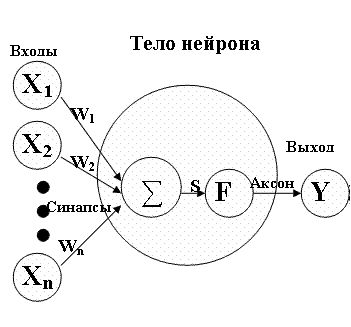
\includegraphics[width=100mm]{neuro.png}
	\caption{Схематическое представление нейрона}
	\label{neuro}
\end{figure}

Именно указанные выше характеристики и стали существенными при создании искусственных нейронных сетей.

Основу нейронной сети составляют как правило однотипные элементы, имитирующие работу биологического нейрона, и называемые обычно так же. Каждый из нейронов в каждый момент времени находится, как и биологический нейрон, в некотором текущем состоянии. Он имеет группу однонаправленных входных связей-синапсов, идущих от входа в сеть или от других нейронов. Кроме того он имеет одну однонаправленную выходную связь-аксон.
\pagebreak

Синаптические связи характеризуются весами $w_i$. Текущее состояние S нейрона равно взвешенной сумме входов:
\begin{equation}
S=\sum_{i=1}^{n}x_i w_i
\end{equation}

В векторном виде это можно записать как $S=XW$, то есть вектор S есть произведение вектора входных значений X на матрицу весов W, где строки соответствуют слоям, а столбцы – нейронам внутри каждого слоя.

Функция S далее преобразуется активационной функцией F и дает выходной сигнал Y нейрона.

Простейшей моделью нейронной сети является однослойный перцептрон. Однослойность означает, что входной сигнал входов $(x_1,x_2,… x_n)$ подается на одну группу нейронов, именуемых слоем нейронной сети, а выходные сигналы этих нейронов поступают сразу на выход сети. Для двуслойной сети выходные сигналы подавались бы не на выход сети, а на вторую группу-слой нейронов, а оттуда на вход. Понятно, что трехслойный нейрон имеет уже три группы-слоя, N-слойный – N групп-слоев и т.д. (см.рисунок \ref{percept}).

\begin{figure}[h!]
	\centering
	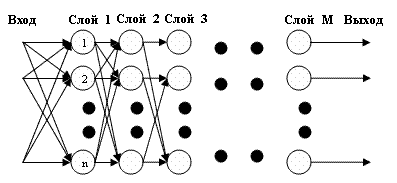
\includegraphics[width=120mm]{percept.png}
	\caption{Схематическое представление перцептрона}
	\label{percept}
\end{figure}

Однослойный перцептрон обнаружил ряд положительных свойств, которые и заставили многих ученых обратить свой взор на исследование нейронных сетей. Главными из обнаруженных свойств перцептрона была способность к обучению и распознаванию. То есть оказалось возможным в ряде случаев установить то, как можно настроить веса синапсов перцептрона, чтобы при различных комбинациях значений входов получать заранее установленные, <<правильные>> значения выходов. То есть однослойный перцептрон оказался способным воспроизводить некоторые математические функции.

Cпособности к распознаванию у многослойных сетей значительно превосходят те же способности у однослойного перцептрона. Зато несколько усложняется процесс обучения этой сети. Под обучением сети мы понимаем процесс настройки весов синапсов, так чтобы выход сети был ожидаемым.

Обучение нейронной сети осуществляется путем последовательного предъявления обучающей выборки, с одновременной подстройкой весов в соответствии с определенной процедурой, пока ошибка настройки по всему множеству не достигнет приемлемого низкого уровня.\cite{le}

После выделения информативных признаков речевого сигнала и представления этих признаков в виде некоторого набора числовых параметров, задача распознавания примитивов речи (фонем и аллофонов) сводится к их классификации при помощи обучаемой нейронной сети. Нейронные сети можно использовать и более высоких уровнях распознавания слитной речи для выделения слогов, морфем и слов.

\subsection{Скрытые модели Маркова}
В качестве метода распознавания большинство современных систем используют метод скрытых марковских моделей\cite{rosti}.  Анализ применимости СММ для распознавания речи приводится в \cite{rabiner_markov}. Использование СММ для распознавания речи базируется на следующих предположениях:  речь может быть разбита на сегменты  (состояния), внутри которых речевой сигнал может рассматриваться как стационарный,  переход между этими состояниями осуществляется мгновенно;  вероятность символа наблюдения, порождаемого моделью,  зависит только от текущего состояния модели и не зависит от предыдущих. Чаще всего используются СММ с тремя состояниями (рисунок \ref{smm_3}).



\begin{figure}[h]	
	\centering
	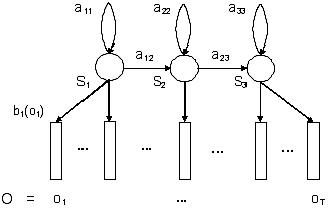
\includegraphics[width=100mm]{smm_3.png}			
	\caption{СММ с тремя состояниями}
	\label{smm_3}
\end{figure}

СММ представляет собой конечный автомат, изменяющий свое состояние в каждый дискретный момент времени t. Переход из состояния $s_{i}$ в состояние $s_{j}$ осуществляется случайным образом с вероятностью $a_{ij}$. В каждый дискретный момент времени модель порождает вектор наблюдений ot (который в конкретной задаче является вектором особенностей, полученным в преобразователе сигнала) с вероятностью $b_{j}(o_{t})$. Распределение плотности вероятности наблюдений моделируется конечной гаусовской смесью с четырьмя компонентами. Каждая такая модель обозначает один из звуков русского языка или отсутствие звука (одна из моделей). Алгоритмы распознавания ключевого слова\cite{hazen} используют эти модели для определения команд в потоке речи. Наиболее часто эта задача решается с помощью метода скользящего окна (sliding window)\cite{bridle} и метода моделей-заполнителей (filler models)\cite{higgins}.

Суть метода скользящего окна заключается в определении вхождения ключевого слова с помощью алгоритма Витерби \cite{couvreur}, который широко применяется для распознавания слитной речи. Этот алгоритм решает следующую задачу: дан вектор наблюдений (о), требуется определить наиболее подходящую последовательность СММ (s) и переходов между их состояниями для этого вектора наблюдений (рисунок \ref{viterbi}). Далее будем называть такую последовательность путем. Под путем здесь следует понимать возможную последовательность СММ и их состояний для определенного участка сигнала. Так, на рисунке \ref{viterbi} изображены все возможные пути для данного участка сигнала и определенной последовательности СММ; утолщенной линией обозначен наиболее вероятный путь. 
\begin{figure}[H]	
	\centering
	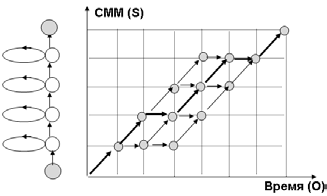
\includegraphics[width=100mm]{viterbi.png}			
	\caption{Пример работы алгоритма Витерби}
	\label{viterbi}
\end{figure}
Так как ключевое слово может начинаться и заканчиваться в любом месте сигнала, то этот метод перебирает все возможные пары начала и конца
вхождения ключевого слова и находит самый вероятный путь для ключевого слова и этого отрезка, как если бы ключевое слово присутствовало в нем. Для каждого найденного вероятного пути ключевого слова применяется функция правдоподобия, основанная на срабатывании, если значение пути, рассчитанное в соответствии с применяемым методом оценки пути, больше предопределенного значения. Часто для оценки пути используется значение вероятности, полученное с помощью алгоритма Витерби.

Главным недостатком такого подхода является то, что он перебирает все возможные варианты вхождения ключевого слова, что создает большую вычислительную сложность. Кроме этого, метод распознавания команды на основе этого алгоритма заключается в применении
его ко всему речевому участку для каждой возможной команды из словаря команд. Такой подход имеет два существенных недостатка:
\begin{enumerate}[1)]
	\item большая вычислительная сложность;
	\item команды могут включать слова, которые плохо распознаются с помощью алгоритма распознавания ключевого слова.
\end{enumerate}
 
Для алгоритмов распознавания ключевого слова слово для распознавания представляется встроенным в инородную речь. На этом основании методы моделей заполнителей \cite{higgins} обрабатывают эту инородную речь с помощью явного моделирования инородной речи за счет второстепенных моделей. Для этого в словарь системы распознавания добавляются «обобщенные» слова. Роль этих слов в том, чтобы любой сегмент сигнала незнакомого слова или неречевого акустического события был распознан системой как одно слово или цепочка
из обобщенных слов. Для каждого обобщенного слова создается и обучается акустическая модель на корпусе данных с соответствующими размеченными сегментами сигнала.На выходе из декодера выдается цепочка, состоящая из слов словаря (ключевых слов) и обобщенных слов. Обобщенные слова затем отбрасываются, и оставшаяся часть цепочки считается результатом распознавания.
Недостатком подхода с использованием слов-заполнителей является высокая вероятность ошибки, когда ключевые слова распознаются как обобщенные. Кроме этого, встает и вопрос об оптимальном выборе алфавита обобщенных слов. Это объясняется тем, что пространство акустических событий, моделируемое альтернативными моделями, очень большое и сложное, поэтому обучение целевых и альтернативных моделей играет важную роль в повышении эффективности метода. В итоге подготовка моделей заполнителей становится нетривиальным процессом, нацеленным на определенный набор команд. Это не дает возможности динамически изменять словарь ключевых слов с сохранением прежних показателей распознавания.\cite{grebnov}

Рассмотренные основные методы распознавания речи на основе скрытых марковских моделей: метод скользящего окна и метод
моделей заполнителей, --- применяются в системах голосового управления и имеют определенные недостатки: первый метод --- большую
вычислительную сложность; второй --- требует подробного дополнительного моделирования посторонней речи. Эти недостатки создают неудобства и мешают применению систем голосового управления на практике. Таким образом, разработка нового алгоритма распознавания речи для систем голосового управления является актуальной задачей в настоящее время. Новый метод не должен требовать трудоемкого дополнительного моделирования посторонней речи и должен иметь низкую вычислительную сложность, которая бы позволяла применять его в режиме реального времени.

\pagebreak

\section[Исследование кепстральных коэффициентов \\ речевых сигналов]{Исследование кепстральных\\ коэффициентов речевых сигналов}
\setcounter{figure}{0} 

В работе \cite{davis} показано, что представление спектра сигнала в виде мел-частотных коэффициентов может успешно применяться в распознавании речи. Значения коэффициентов в шкале мел могут быть получены, анализируя значения коэффициентов в шкале Герц с последующим переходом при использовании выражения:
\begin{equation}
	B(f)=1125\ln(1+f/700)
	\label{eq:mel}
\end{equation}
где  $f$ --- значение частоты в Герцах;\\
$B(f)$ --- значение частоты в мел, соответствующее частоте в Герцах $f$.

Тогда для оценки значений мел-частотных кепстральных коэффициентов на первом этапе необходимо оценить значения трансформанты Фурье анализируемого фрагмента сигнала вида:
\begin{equation}
	X_{k} =\sum_{n=0}^{N-1}x_{n}e^{\frac{-2\pi i}{N} kn},  \;\; 0\le k<N_f,
\end{equation}
где  $x_n$ --- анализируемый отрезок сигнала, длительностью $N$ отсчетов, $N_f$ --- количество точек Фурье.

При оценке логарифмов значений трансформант Фурье предлагается использовать треугольную оконную функцию вида:
\begin{equation}
	H_{m}=
	\begin{cases}
		0,&k<f_{m-1}\\ 
		\frac{(k-f_{m-1})}{(f_{m}-f_{m-1})},&f_{m-1} \leq k < f_{m}\\ 
		\frac{(f_{m+1}-k)}{(f_{m+1}-f[m])},&f_{m} \leq k \leq f_{m+1}\\ 
		0,&k > f_{m+1}
	\end{cases}
	\label{eq:window}
\end{equation}
где $f_m$ – граничная частота m-го окна.

Окна предлагается располагать равномерно относительно шкалы мел, т.е. в шкале мел граничные частоты определяются с использованием выражения:
\begin{equation}
B(f_{m})=B(f_1)+m\frac{B(f_{\text{в}})-B(f_{1})}{M+1}, \; \; 0 \leq m < M,
\end{equation}
где $m$ -- номер треугольного окна, \\$M$ -- число треугольных окон, равномерно расположенных в шкале мел,\\ $B(f_1)$ -- нижнее значение частоты в шкале мел, рассчитанное с использованием выражения (\ref{eq:mel}),\\ $B(f_{\text{в}})$ –- верхнее значение частоты в шкале мел, рассчитанное с использованием выражения (\ref{eq:mel}).

Тогда в шкале Герц граничные частоты имеют вид:
\begin{equation}
f_m=\frac{N}{F_s}\cdot 700 \cdot (e^{B(f_m)/1125}-1),
\end{equation}
где  $B(f_m)$ -- граничные значения частоты в мел.

Для оценки кепстральных коэффициентов необходимо оценить значения логарифмов результата дискретного преобразования Фурье:
\begin{equation}
S_m=\ln(\sum_{k=0}^{N-1}|X_k|^2 H_{m,k}), \; \; 0\leq m \le M,
\label{eq:cepstr}
\end{equation}
где $X_k$ –- значения трансформанты Фурье,\\
$M$ – число треугольных окон, равномерно расположенных в шкале мел,\\
$H_{m,k}$ -– значения оконной функции вида (\ref{eq:window}).

Затем к полученным результатам применяются дискретное косинусное преобразование:
\begin{equation}
c_n=\sum_{m=0}^{M-1}S_m cos(\pi n(m+\frac{1}{2})/M), \; \; 0\leq n \le M,
\end{equation}
где  $M$ – количество треугольных окон, равномерно распределенных в шкале мел,\\
$S_m$ – значение результата логарифмирования вида (\ref{eq:cepstr}).

Исследование особенностей значений кепстральных коэффициентов для различных звуков русской речи показало, что распределение кепстральных коэффициентов зависит от типа звука. На рисунке \ref{sounds_mfcc} представлены наборы кепстральных коэффициентов для трех реализаций звука <<а>> и звука <<и>>. Можно заметить, что для разных реализаций одного звука наборы коэффициентов схожи.

Таким образом, эта особенность может быть использована при разработке решающих функций распознавания речевых сигналов.

В проведенных экспериментах анализировались отрезки сигнала длиной в 256 отсчетов (16 мс при используемой частоте дискретизации 16 кГц) с перекрытием в 128 отсчетов, с целью обеспечения относительной стационарности анализируемого речевого отрезка. Количество точек Фурье устанавливалось равным длине отрезка.
\pagebreak

\begin{figure}[!ht]
	\centering
	\begin{subfigure}{0.49\textwidth}
	\centering
	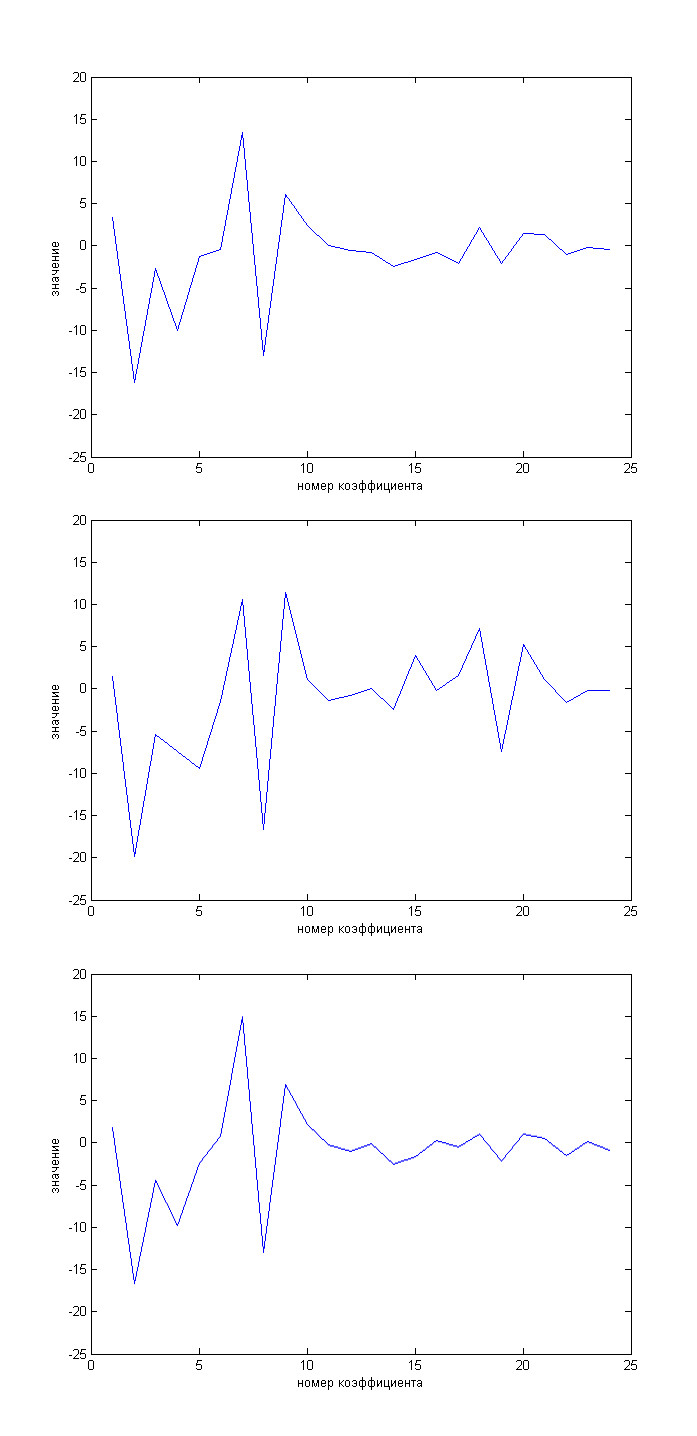
\includegraphics[width=.99\textwidth]{a_mfcc.png}
	\caption{}
	\label{a_mfcc}
	\end{subfigure}
	\begin{subfigure}{0.49\textwidth}
	\centering
	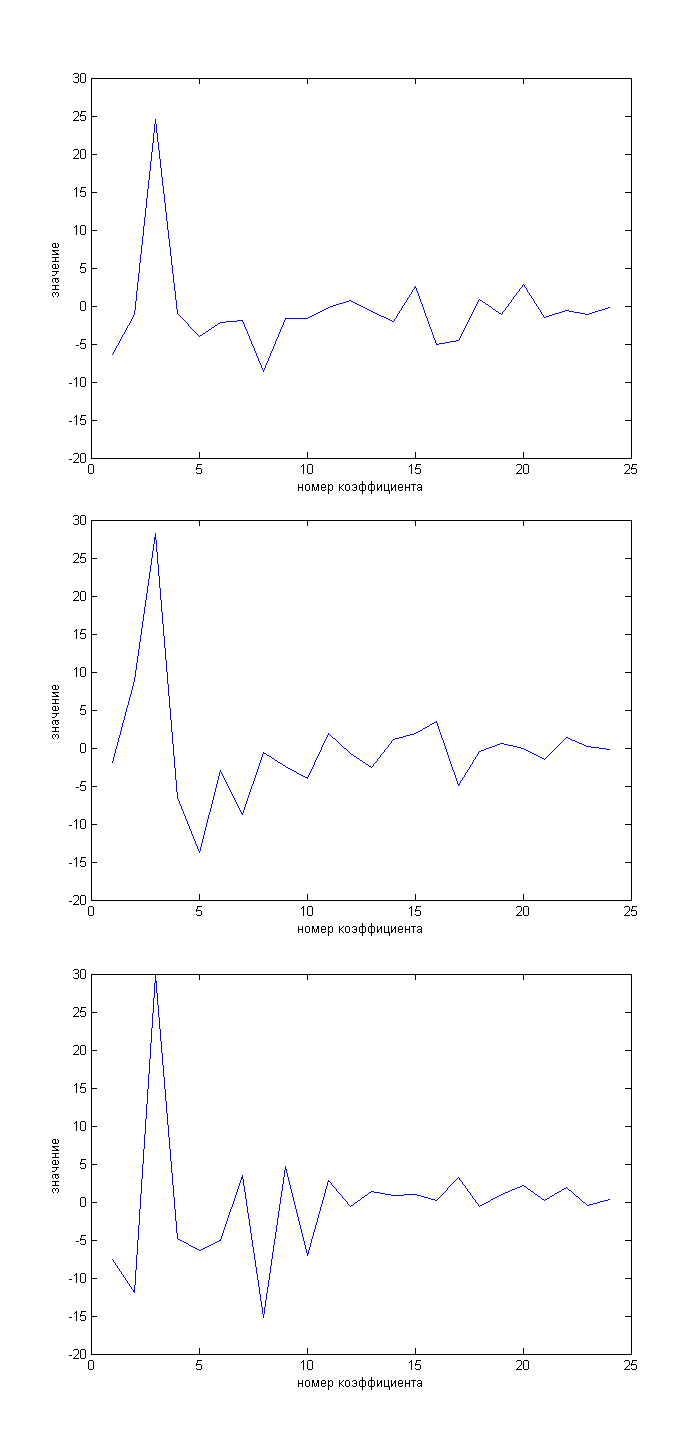
\includegraphics[width=.99\textwidth]{i_mfcc.png}
	\caption{}	
	\label{i_mfcc}
	\end{subfigure}
	\caption{Мел-кепстральные коэффициенты звуков: \\ а) звук <<а>>; \\ б) звук <<и>>}
	\label{sounds_mfcc}
\end{figure}


Количество используемых коэффициентов установлено равным 24 на основании рекомендаций, приведенных в \cite{spokenlang}. Также было исследовано влияние количества используемых коэффициентов на точность распознавания речевых сигналов. В эксперименте рассчитывались все 24 коэффициента, а затем для описания сигнала в алгоритме распознавания использовались $N_k$ коэффициентов. На рисунке \ref{mfcc_number} сплошной линией изображен график зависимости вероятности ошибки от количества коэффициентов, взятых с 1 по $N_k$. Пунктирной линией -- с 24 по $(24-N_k)$

\begin{figure}[h]
	\centering
	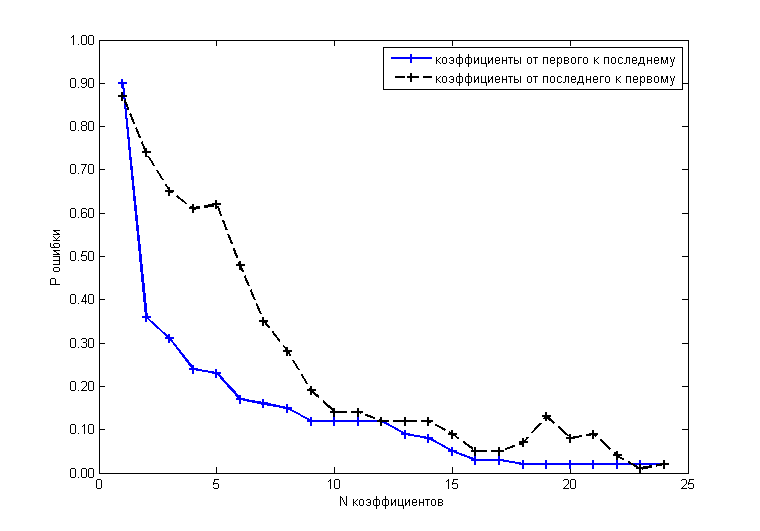
\includegraphics[width=150mm]{decrease_legend.png}
	\caption{Зависимость вероятности ошибки распознавания от количества используемых коэффициентов}
	\label{mfcc_number}
\end{figure}

Исходя из результатов эксперимента, можно предположить возможность использования меньшего количества коэффициентов в качестве описания сигнала, что позволяет уменьшить размер хранимого словаря и ускорить выполнение алгоритма распознавания.

\pagebreak

\section[Исследование алгоритма динамического \\ трансформирования времени (DTW)]{Исследование алгоритма динамического \\трансформирования времени (DTW)}
\setcounter{figure}{0} 
Одной из основных проблем распознавания речевых сигналов является тот факт, что одно и то же сочетание звуков, произнесенных несколько раз или же различными дикторами, может значительно отличаться по многим критериям: длительности, скорости произведения, форме огибающей, амплитуде и т.д. При разработке алгоритма распознавания с ограниченным словарем необходимо разработать такую решающую функцию, которая будет незначительно зависеть от этих критериев.
Простейшим способом распознавания речевых сигналов при использовании ограниченного словаря видится сравнение анализируемого фрагмента сигнала с базой эталонов и принятие решения на основе наименьшего отклонения от какого-либо эталона. При этом наряду с разработкой базы эталонов, возникает проблема, связанная с тем, что одно и то же сочетание звуков может иметь различную длительность. Использование алгоритма динамического трансформирования времени позволяет избежать этой проблемы.
Алгоритм динамического трансформирования времени (англ. Dynamic Time Warp или DTW) вычисляет оптимальную последовательность трансформации (деформации) времени между двумя временными рядами. Алгоритм вычисляет оба значения деформации между двумя рядами и расстояние между ними.\cite{sakoe}

Предположим, что есть две числовые последовательности $A= a_{1}, a_{2}, \dots, a_{I}$ и $B=b_{1}, b_{2}, \dots, b_{J}$. Длина двух последовательностей может быть различной.

Временные различия между A и B могут быть описаны с помощью некоторой последовательности $c=(i,j)$:
\begin{equation}
	F=c(1),c(2)\dots,c(k),\dots,c(K)
	\label{eq:F}
\end{equation}
где $c(k)=(i(k),j(k))$.
Данная последовательность представляет собой функцию, которая позволяет отобразить временную ось A на временной оси B. Назовем ее функцией деформации. \cite{sakoe}

\begin{figure}[ht]	
	\centering
	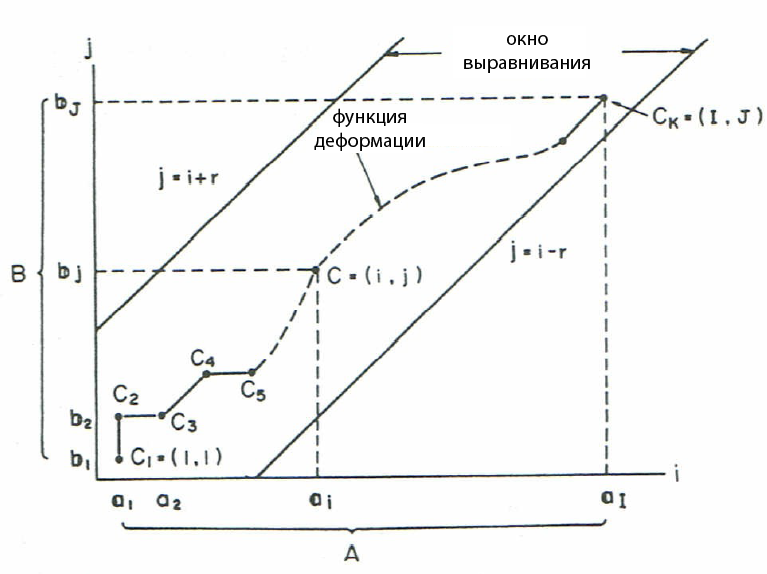
\includegraphics[width=120mm]{sakoe1.png}			
	\caption{Функция деформации и окно выравнивания}
	\label{sakoe1}
\end{figure}

Алгоритм начинается с расчета локальных расстояний между элементами двух последовательностей. Самым распространенным способом для вычисления расстояний является метод, рассчитывающий модуль разности между значениями двух элементов (евклидова метрика):
\begin{equation}
	d(i,j)=|a_{i}-b_{j}|, i=1..I, j=1..J, 	
\end{equation}
где I, J – длительности соответственно первого и второго сигнала.

Для сравнения речевых сигналов евклидова метрика оказалась неэффективной, поэтому в рамках данной работы при реализации алгоритма динамического трансформирования используются коэффициенты корреляции Пирсона, рассчитанные для кепстральных коэффициентов отрезков сигнала:
\begin{equation}
	d(i,j)=1-\frac{\sum_{k-1}^{M}c1_{i,k}\cdot c2_{i,k}}{\sqrt{\sum_{k-1}^{M}c1_{i,k}^2 \cdot c2_{i,k}^2}}, \; \; 1 \leq i \leq I, \; 1 \leq j \leq J,
	\label{eq:pirson}
\end{equation}
где с1, с2 – кепстральные коэффициенты соответственно первого и второго сигнала;\\
I, J – длительности соответственно первого и второго сигнала;\\
М – количество кепстральных коэффициентов, используемых для анализа.

В результате получаем матрицу расстояний, имеющую I строк и J столбцов общих членов:
\begin{equation}
	d(c)=d(i,j)
\end{equation}

Взвешенная сумма значений метрик в точках, принадлежащих функции деформации F
\begin{equation}
	E(F)=\sum_{k=1}^{K}{d(c(k))\cdot w(k)},	
\end{equation}
где $w(k)$ - неотрицательный весовой коэффициент;
является мерой доброкачественности функции F. Она принимает минимальное значение, когда функция F оптимально выравнивает временные различия между A и B. Минимальное остаточное расстояние между A и B, которое остается после устранения временных различий, может служить мерой различия речевых последовательностей A и B
\begin{equation}
	Dist(A,B)=min_F\left[\frac{\sum_{k=1}^{K}{d(c(k))\cdot w(k)}}{\sum_{k=1}^{K}{w(k)}}\right]
	\label{eq:dist}
\end{equation}

Существует три условия, налагаемых на DTW алгоритм для обеспечения быстрой конвергенции:

\begin{enumerate}[1)]
 \item Монотонность – путь никогда не возвращается, то есть: оба индекса, $i$ и $j$, которые используются в последовательности, никогда не уменьшаются. 

 \item Непрерывность – последовательность продвигается постепенно: за один шаг индексы $i$ и $j$, увеличиваются не более чем на 1.

 \item Предельность – последовательность начинается в $(1,1)$ и заканчивается в $(I,J)$.
 \end{enumerate}

Также в работе \cite{sakoe} предлагается ввести дополнительное условие, названное <<окно выравнивания>>, определяющее дополнительные границы, в которых может лежать функция F (см. рисунок \ref{sakoe1}).

С учетом данных граничных условий, нахождение минимальной функции F является типичной задачей динамического программирования.

Блок-схема реализованного алгоритма сравнения двух наборов кепстральных коэффициентов, соответствующих речевым сигналам, приведена на рисунке \ref{block1}. Алгоритм выполняет поиск кратчайшего пути в матрице коэффициентов корреляции, построенной с помощью выражения (\ref{eq:pirson}), между элементами $d(1,1)$ и $d(I,J)$. В соответствии с принципом динамического программирования задача разбивается на элементарные операции, в данном случае для каждой точки $d(i,j)$, находящейся в окне выравнивания выбирается одно из трех возможных направлений перехода: $D=d(i+1,j)$, $D=d(i,j+1)$ или $D=d(i+1,j+1)$, такое чтобы накопленная сумма значений $S=d(i,j)+D$ была минимальной. Полученное минимальное значение $S$ записывается в выбранный для перехода элемент, таким образом происходит накопление суммы. То есть в элемент $d(I,J)$ будет записана сумма значений матрицы $d$, лежащих в точках кратчайшего пути. Чтобы использовать эту сумму в качестве меры схожести двух наборов коэффициентов, необходимо произвести ее нормировку. Для этого $d(I,J)$ делится на длину полученного кратчайшего пути, то есть количество шагов.
\pagebreak
\begin{figure}[H]	
	\centering
	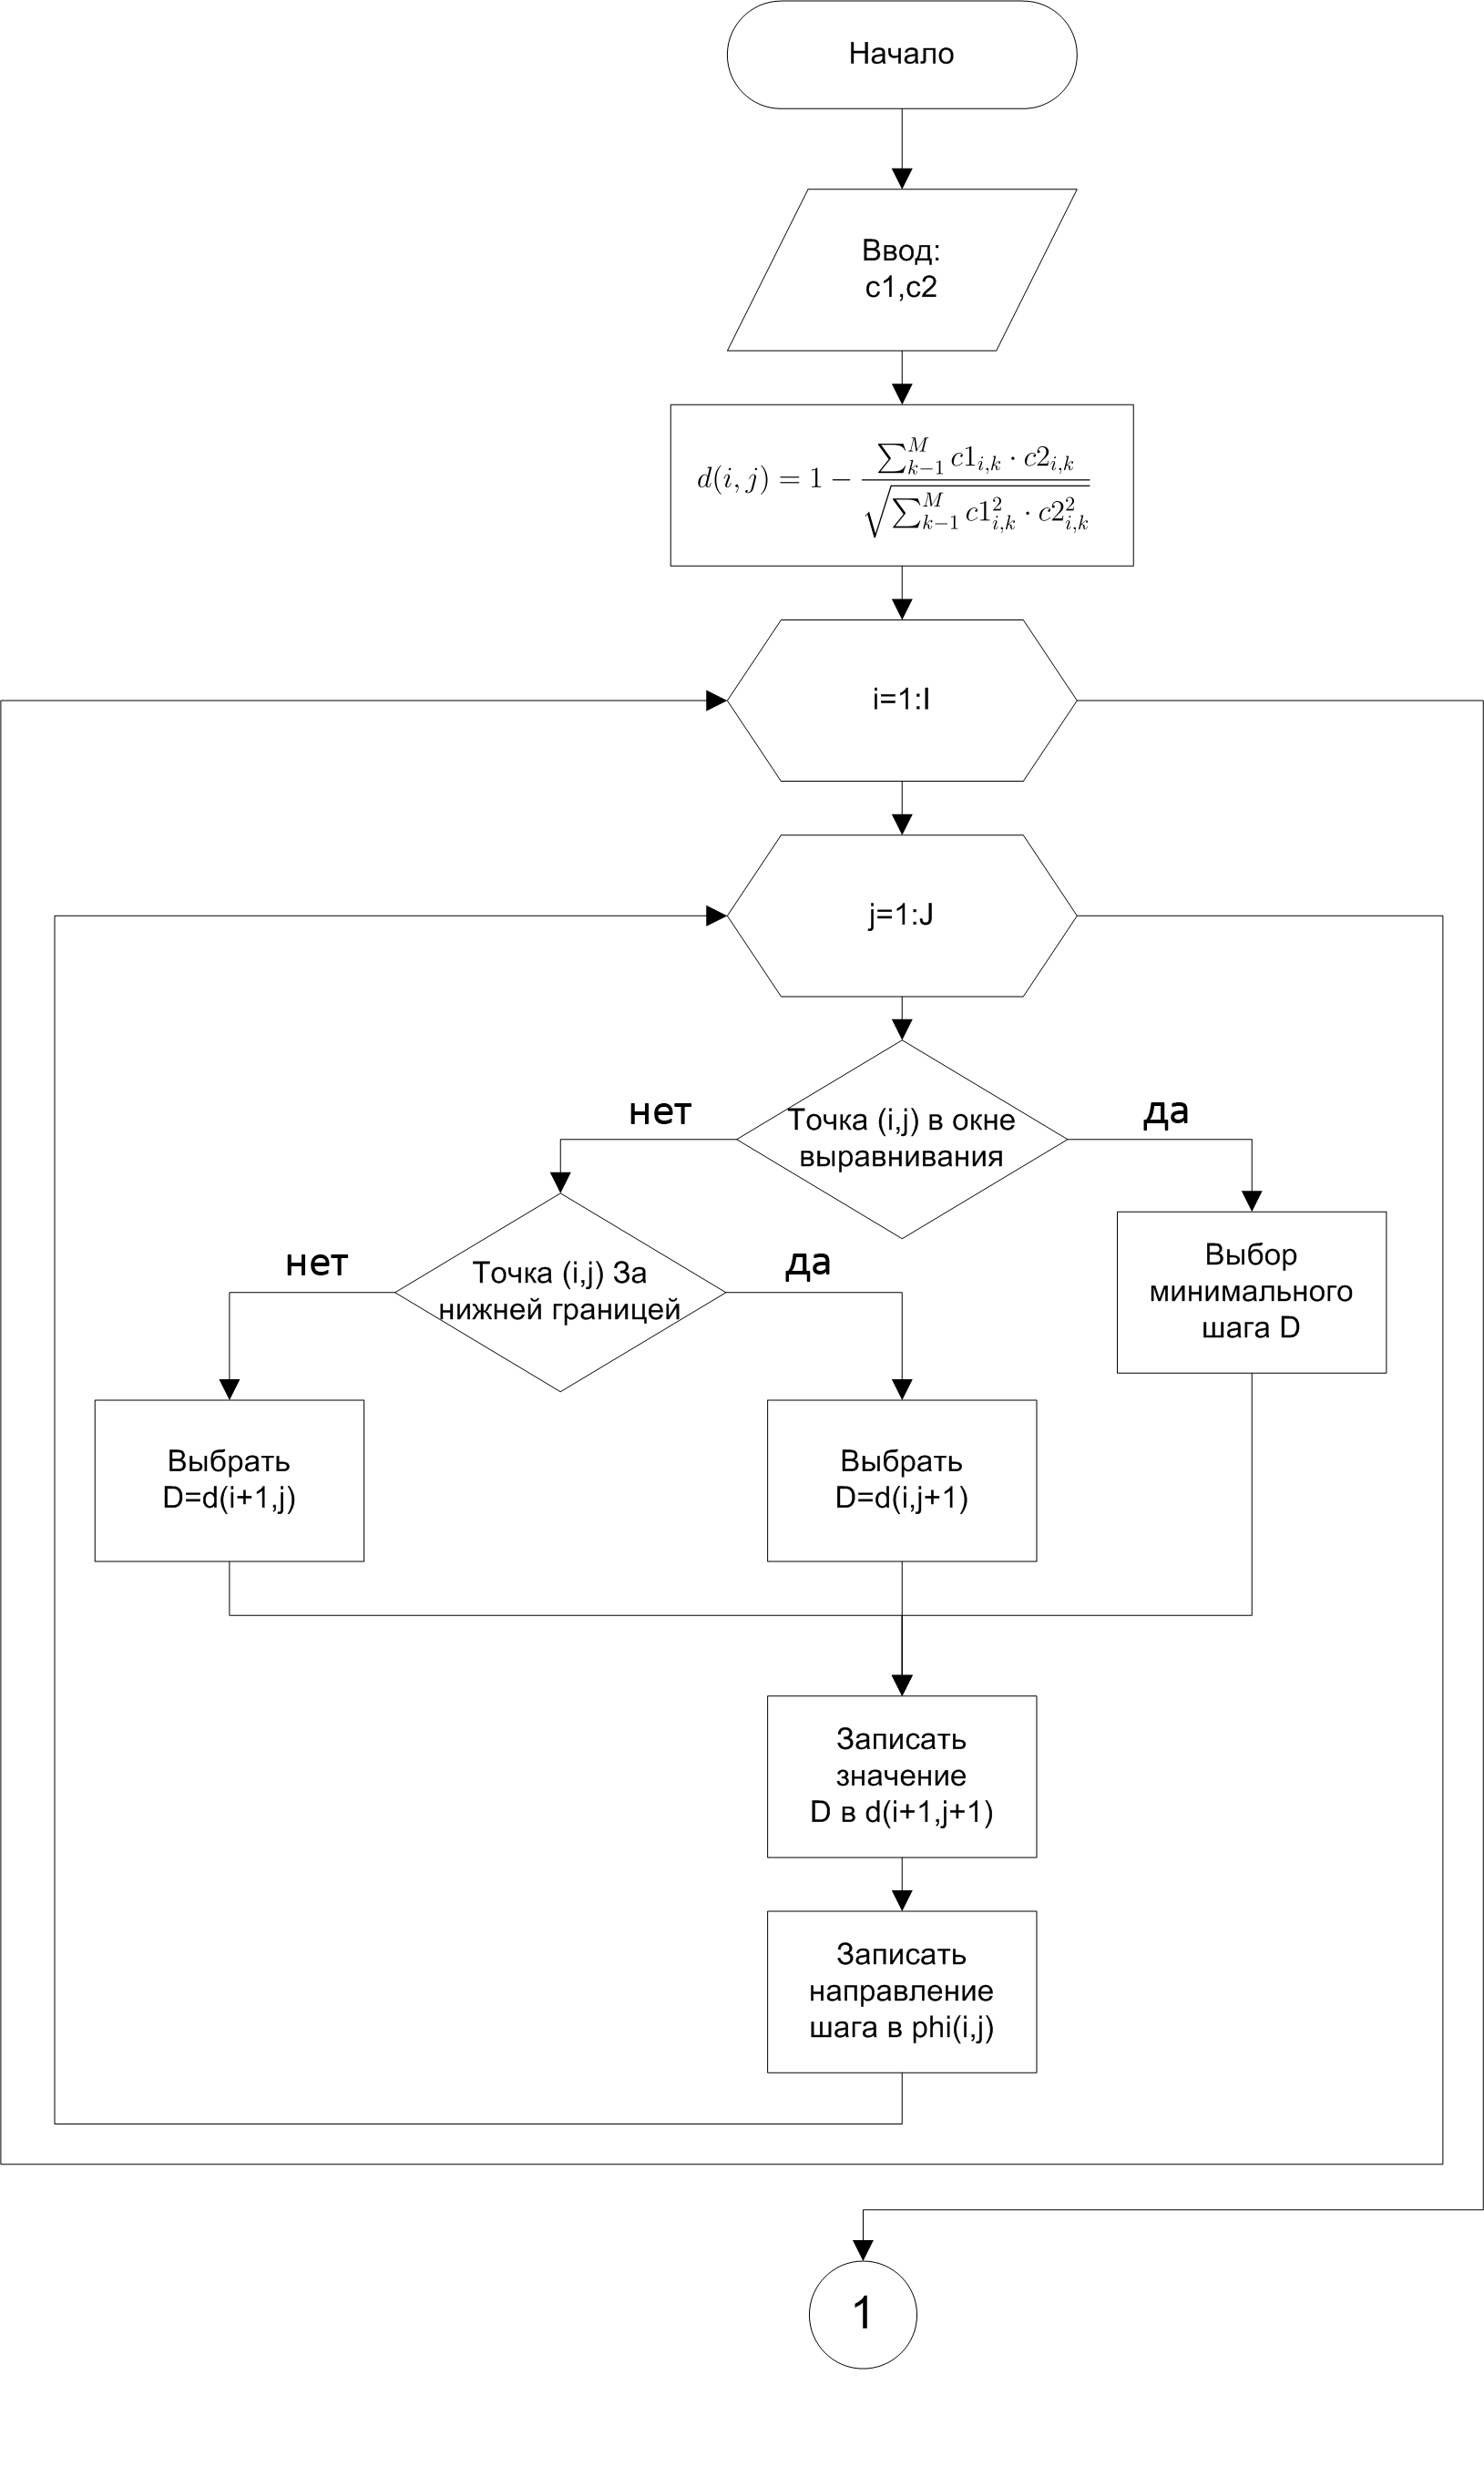
\includegraphics[width=150mm]{block1.png}			
	\caption{Блок-схема DTW алгоритма}
	\label{block1}
\end{figure}
\addtocounter{figure}{-1}
\begin{figure}[H]	
	\centering
	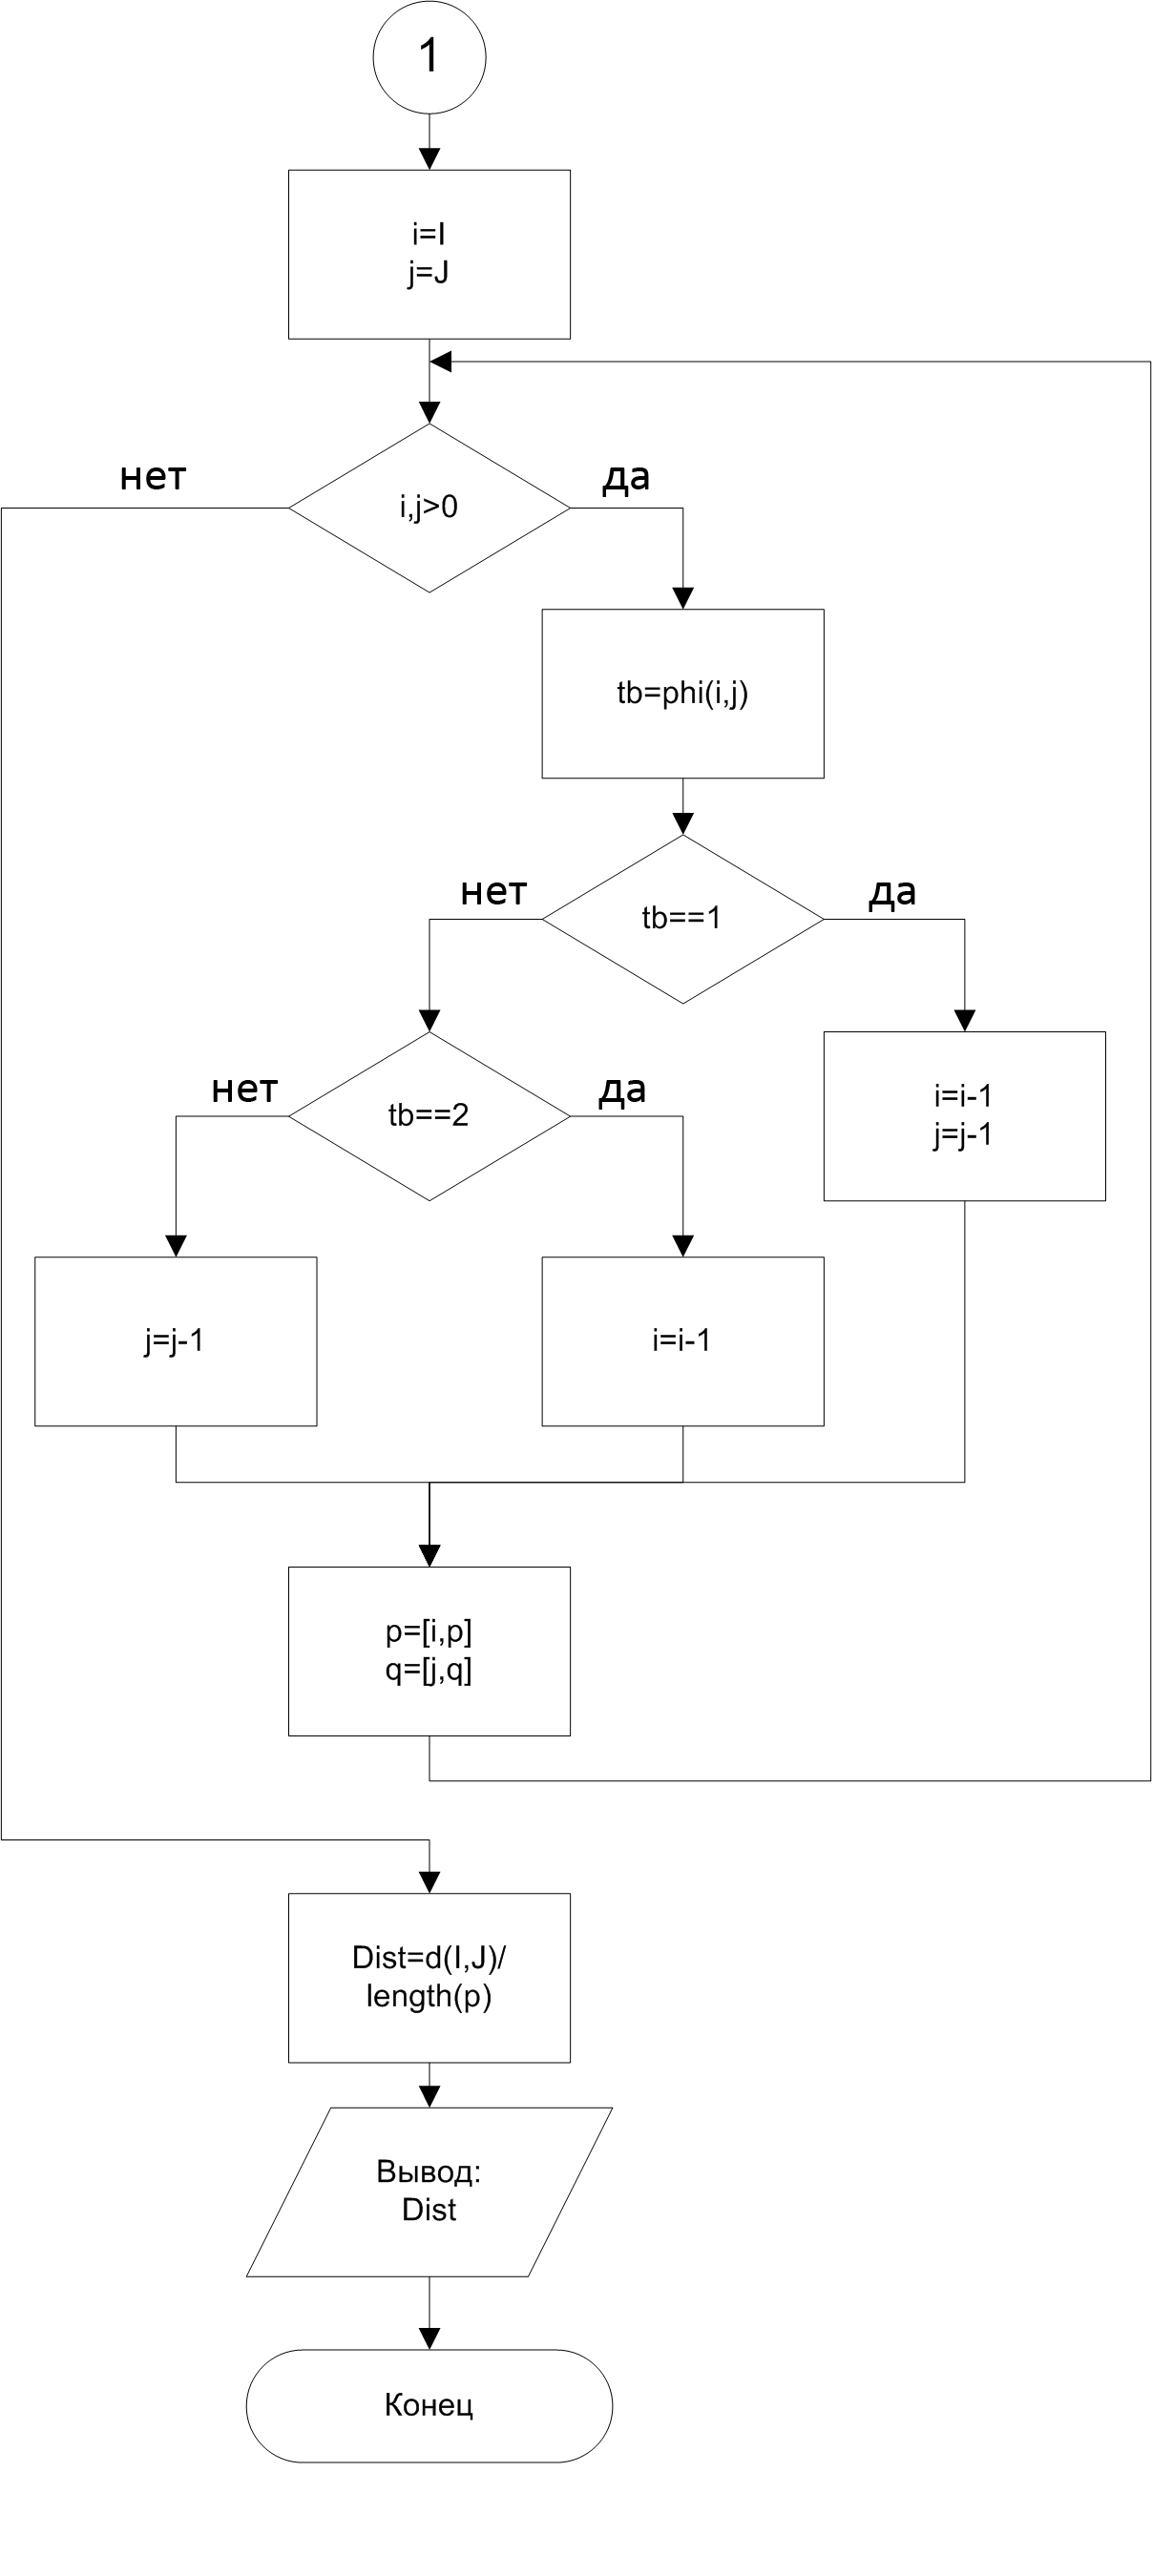
\includegraphics[width=110mm]{block2.png}			
	\caption{(продолжение)}
	\label{block2}
\end{figure}

Пример найденной таким образом функции деформации F, представлен на рисунке \ref{d_matrix}

\begin{figure}[h]	
	\centering
	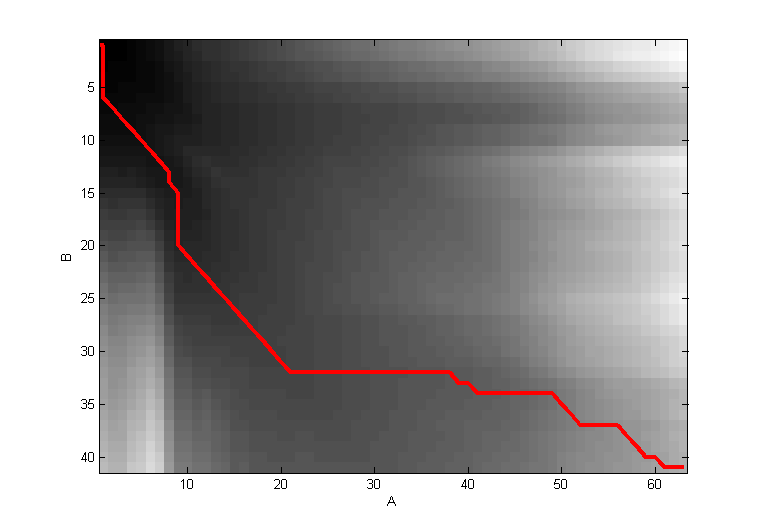
\includegraphics[width=120mm]{d_matrix.png}			
	\caption{Функция \textit{F} вида (\ref{eq:F}), наложенная на матрицу \textit{d}}
	\label{d_matrix}
\end{figure}

Вычислительная сложность реализованного алгоритма составляет порядка $O(IJ)$, возможно, сложность может быть уменьшена оптимизацией алгоритма.

С помощью данного алгоритма производится сравнение анализируемого сигнала с сохраненными в памяти компьютера эталонами. В результате выбирается пара с минимальной дистанцией и делается вывод о соответствии сигнала слову из словаря. На рисунке \ref{dist_4} представлен результат оценки меры различий вида (\ref{eq:dist}) для слова «четыре».

Анализ рисунка показывает, что наименьшее значение отличия наблюдается для слова «четыре». Таким образом, в данном случае, алгоритм принимает верное решение.

\begin{figure}[H]	
	\centering
	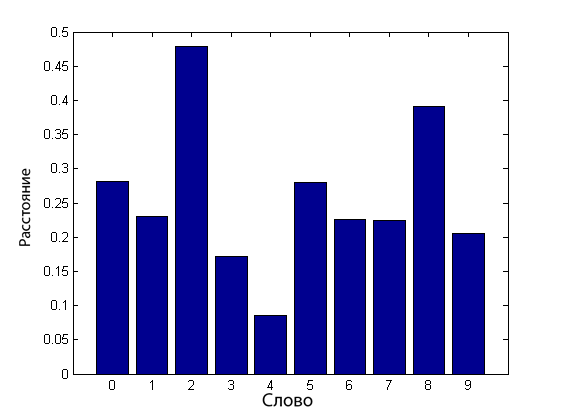
\includegraphics[width=120mm]{dist_4.png}
	\caption{Значения меры отличий для слова «четыре»}
	\label{dist_4}
\end{figure} 

\begin{figure}[H]	
	\centering
	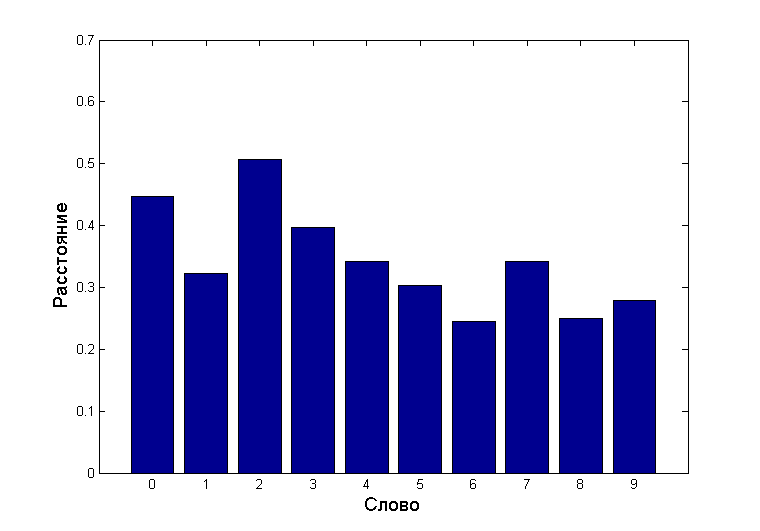
\includegraphics[width=120mm]{err_8.png}			
	\caption{Значения меры отличий для ошибочно распознанного слова <<восемь>>}
	\label{dist_error8}
\end{figure}

Для исследования данного алгоритма была составлена база эталонов из 10 слов (числительные от 0 до 9). В качестве исходного сигнала использовались записи речевого сигнала с частотой дискретизации 16 кГц и разрядностью кода 16 бит. Исследование вероятностей ошибочного принятия решения осуществлялось на основе анализа 10 повторений этих же числительных тем же диктором (100 образцов). В результате, на 100 повторений было обнаружено 2 ошибки распознавания, что позволяет говорить о достаточной степени точности выбранного алгоритма.

Диаграммы значений меры различий для ошибочных решений приведены на рисунках. В данном случае алгоритм ошибочно опознал слово <<восемь>> как слово <<шесть>> (рисунок \ref{dist_error8}) и слово  <<пять>> как слово <<три>> (рисунок \ref{dist_error5}).




\begin{figure}[h]	
	\centering
	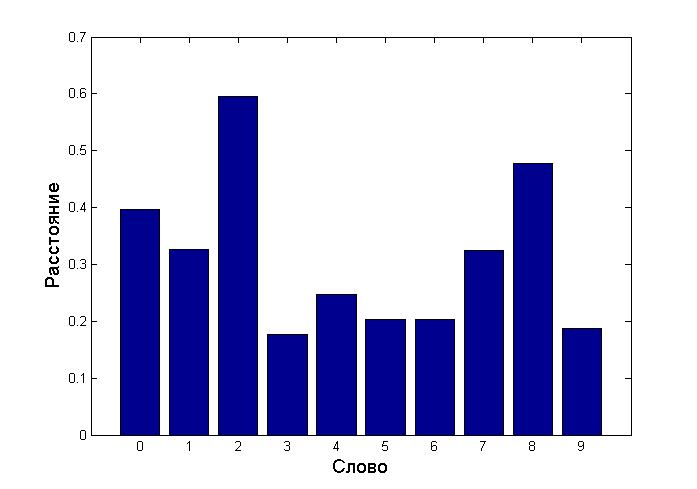
\includegraphics[width=120mm]{err_5.png}			
	\caption{Значения меры отличий для ошибочно распознанного слова <<пять>>}
	\label{dist_error5}
\end{figure}

К достоинствам выбранного алгоритма можно отнести достаточно высокую точность распонавания при работе с небольшим словарем, относительно небольшую сложность реализации и устойчивость к различиям в скорости произношения анализируемых слов. Однако, данный алгоритм обладает и рядом недостатков, таких как ограниченность размера используемого словаря, чувствительность к точности выделения слова из речевого потока и влиянию шумов.


Так диаграмма значений меры различий для произнесенного слова <<четыре>>, представленная на рисунке \ref{clear_4}, меняется при добавлении к сигналу аддитивного белого гауссовского шума с отношением сигнал-шум, равным 60 дБ, к виду, представленному на рисунке \ref{60db_4}. Из анализа диаграмм ясно, что принятие решения затруднено влиянием шума. Уменьшение отношения сигнал-шум до 40 дБ приводит диаграмму к виду, показанному на рисунке \ref{40db_4}, где можно видеть ошибочно принятое решение.

\begin{figure}[H]	
	\centering
	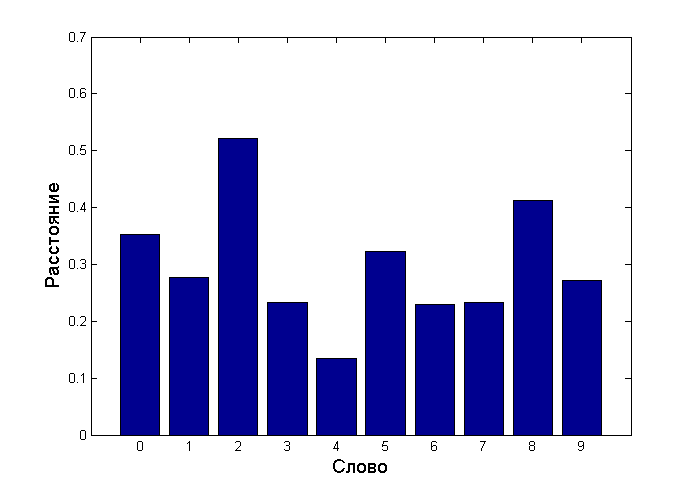
\includegraphics[width=120mm]{clear_4.png}			
	\caption{Значения меры отличий для слова <<четыре>> без влияния шумов}
	\label{clear_4}
\end{figure}

\begin{figure}[H]	
	\centering
	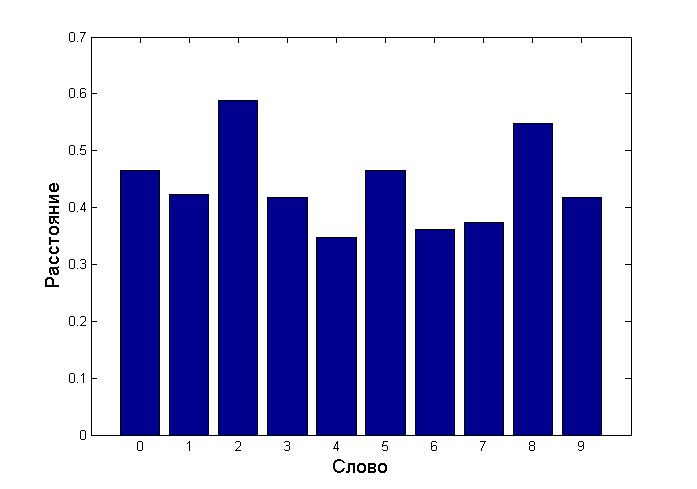
\includegraphics[width=120mm]{60db_4.png}			
	\caption{Значения меры отличий для слова <<четыре>> \\ (отношение сигнал-шум 60 дБ)}
	\label{60db_4}
\end{figure}

\begin{figure}[H]	
	\centering
	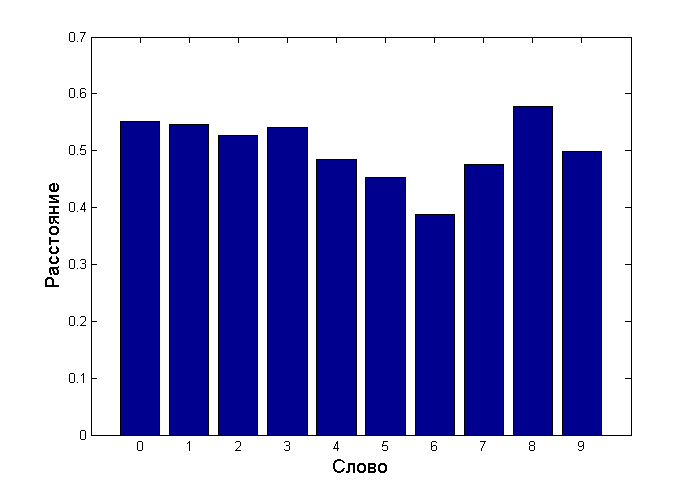
\includegraphics[width=120mm]{40db_4.png}			
	\caption{Значения меры отличий для слова <<четыре>> \\ (отношение сигнал-шум 40 дБ)}
	\label{40db_4}
\end{figure}

Аналогичный эксперимент был проведен для слова <<шесть>>. Результаты представлены на рисунках \ref{clear_6}, \ref{60db_6}, \ref{40db_6}, \ref{20db_6}

\begin{figure}[H]	
	\centering
	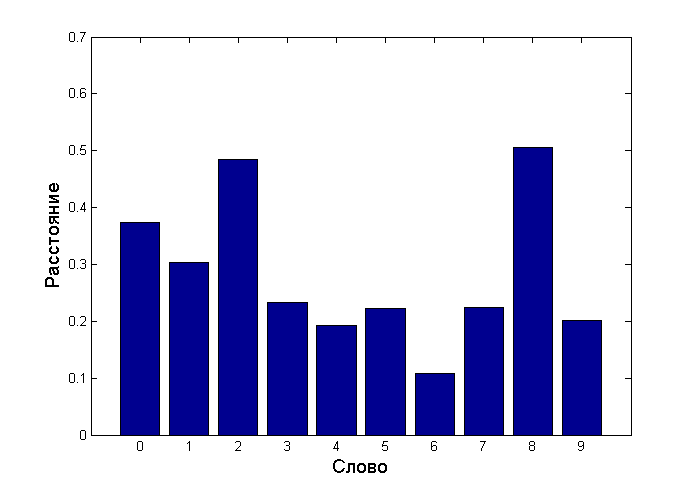
\includegraphics[width=120mm]{clear_6.png}			
	\caption{Значения меры отличий для слова <<шесть>> без влияния шумов}
	\label{clear_6}
\end{figure}

\begin{figure}[H]	
	\centering
	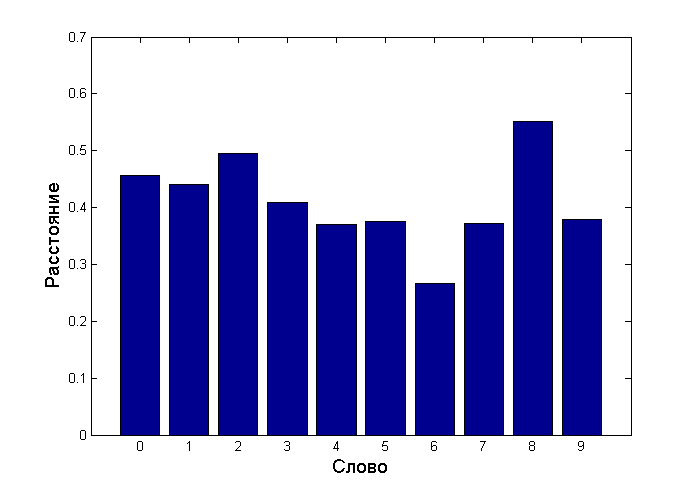
\includegraphics[width=120mm]{60db_6.png}			
	\caption{Значения меры отличий для слова <<шесть>> \\ (отношение сигнал-шум 60 дБ)}
	\label{60db_6}
\end{figure}

\begin{figure}[H]	
	\centering
	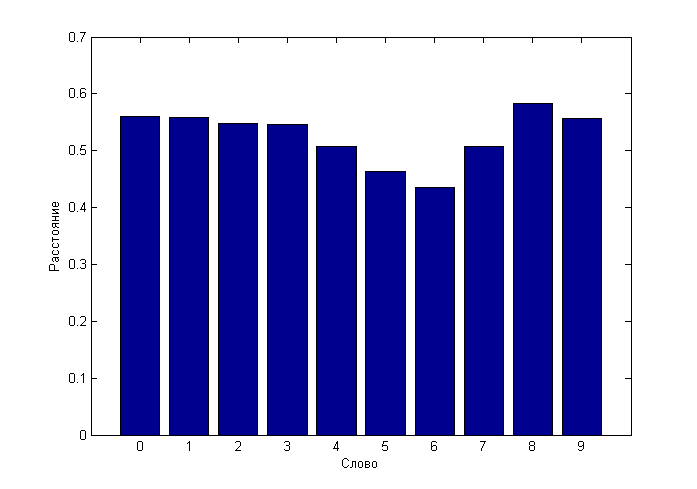
\includegraphics[width=120mm]{40db_6.png}			
	\caption{Значения меры отличий для слова <<шесть>> \\ (отношение сигнал-шум 40 дБ)}
	\label{40db_6}
\end{figure}

\begin{figure}[H]	
	\centering
	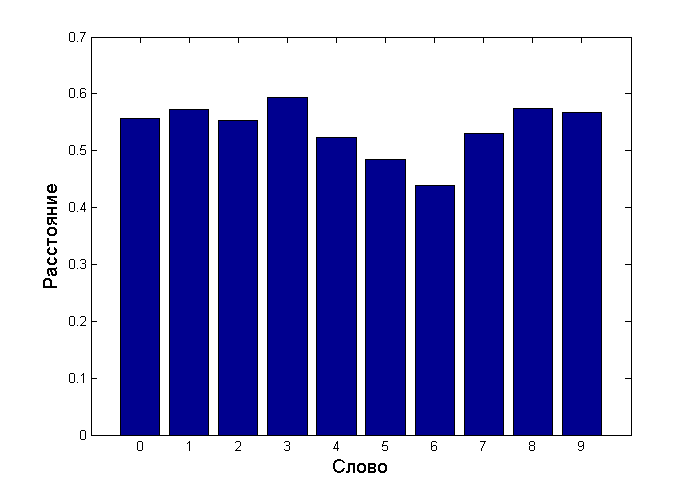
\includegraphics[width=120mm]{20db_6.png}			
	\caption{Значения меры отличий для слова <<шесть>> \\ (отношение сигнал-шум 20 дБ)}
	\label{20db_6}
\end{figure}

Из рисунков видно, что влияние аддитивного белого гауссовского шума на распознавание слова <<шесть>> меньше, чем для слова <<четыре>>. Такой результат можно объяснить изначальным наличием в сигнале шумоподобных составляющих, соответствующих звукам <<ш>> и <<с>>.

Был проведен экспериментальный анализ зависимости точности распознавания от значения отношения сигнал-шум. Для этого вся база из 100 записанных слов сравнивалась с имеющимися эталонами, при этом в каждой итерации из 100 сравнений к анализируемым речевым сигналам добавлялся аддитивный гауссовский белый шум различной мощности. Результаты эксперимента приведены на рисунке \ref{snr-err}

\begin{figure}[H]	
	\centering
	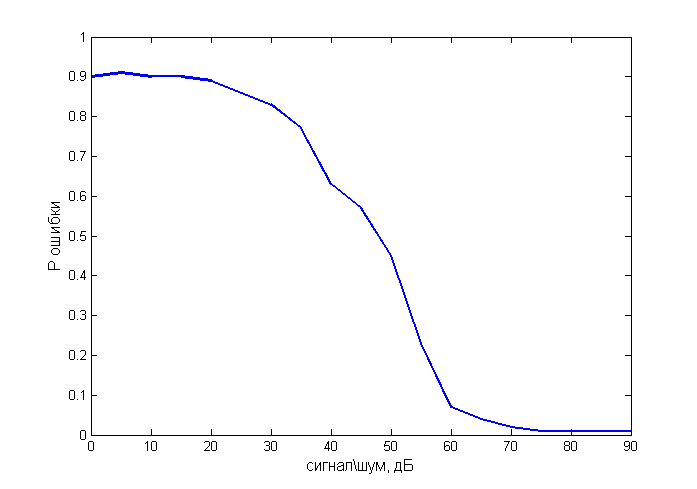
\includegraphics[width=120mm]{snr-err.png}			
	\caption{Зависимость вероятности ошибки распознавания от отношения сигнал-шум}
	\label{snr-err}
\end{figure}

Из рисунка видно, что даже при относительно высоких значениях отношения сигнал-шум, когда человек еще уверенно воспринимает произнесенные слова, используемый алгоритм показывает неприемлемо высокую вероятность ошибки распознавания.
\pagebreak

\section*{Заключение}
\addcontentsline{toc}{section}{ЗАКЛЮЧЕНИЕ}

В ходе выполнения данной работы были решены все поставленные задачи. Изучены существующие подходы к решению проблемы распознавания устной речи, выбран, реализован и исследован один из применяемых алгоритмов.

Модели речевых сигналов, использующиеся в системах распознавания речи, основываются на теории речеобразования и речевосприятия, поэтому основные теоретические понятия рассмотрены в первом разделе данной работы. Также в работе выполнен обзор основных методов, используемых для анализа сигналов в современных системах распознавания речи.

Из существующих алгоритмов распознавания устной речи для подробного анализа выбран один --- алгоритм динамического трансформирования времени (DTW), основанный на принципах динамического программирования. Выбор данного алгоритма объясняется возможностью его практической реализации в рамках выпускной квалификационной работы, а также его непосредственной применимостью к задаче распознавания речевых команд в системах с небольшим словарем (до 50 слов). Другие известные алгоритмы,  использующие, например, скрытые модели Маркова или нейронные сети, обычно, являются частью более сложных систем, реализация которых требует существенных затрат.

Исследованный в работе алгоритм показал достаточно высокую точность (98\%). При этом минимизировано влияние на точность распознавания громкости (за счет нормирования) и скорости произнесения (за счет методов динамического программирования). Наряду с достоинствами были выявлены и основные недостатки алгоритма, такие как низкая устойчивость к воздействию шумов. Вопросы дикторозависимости, которые не рассматривались в данной работе, могут быть предметом дальнейших исследований.

\pagebreak
\begin{thebibliography}{99}

\bibitem{sakoe}
Sakoe, H. Dynamic programming optimization for spoken wordrecognition/ H. Sakoe, S. Chiba. – IEEE Trans. Acoust. Speech Signal Process., Vol. ASSP-26, No.1, Feb. 1978.
\bibitem{agran}
Аграновский, А. В. Теоретические аспекты алгоритмов обработки и классификации речевых сигналов [Текст]/ А. В. Аграновский, Д. А. Леднов – М.: Радио и связь, 2004. --- 164 с.
\bibitem{rabiner1}
Рабинер, Л. Р. Цифровая обработка речевых сигналов [Текст]/ Л.Р. Рабинер, Р.Ф. Шафер. – М.: Радио и связь, 1981. – 496 с.
\bibitem{sorokin}
Сорокин, В. Н. Теория речеобразования [Текст]/ В. Н. Сорокин – М.: Радио и связь, 1985. – 312 с.
\bibitem{davis}
Davis, S. Comparison of Parametric Representations for Monosyllable Word Recognition in Continuously Spoken Sentences/ S. Davis, S.P. Mermelstein. – IEEE Trans. on Acoustics, Speech and Signal Processing, 1980.
\bibitem{mazurenko}
Мазуренко, И. Л. Компьютерные системы распознавания речи. [Текст]/ И. Л. Мазуренко - М.: Интеллектуальные системы, 1998.
\bibitem{bondarko}
Основы общей фонетики. [Текст]/ Л. В. Бондарко, Л. А. Вербицкая, М. В. Гордина. --- 4-е изд. - СПб: Академия, 2004. --- 160 с.
\bibitem{rabiner_eng}
Rabiner, L. Fundamentals of speech recognition [Текст]/ L. R. Rabiner, B. Juang --- Prentice-Hall, 1993.
\bibitem{gorelik}	
Горелик, А. Л. Методы распознавания [Текст]/ А. Л. Горелик, В. А. Скрипкин --- 4-е изд. --- М.: Высшая школа, 2004. --- 262 с.
\bibitem{vincuk}
	Винцюк, Т. К. Анализ, распространение и интерпретация речевых сигналов [Текст]/ Т. К. Винцюк. - Киев: Наукова думка, 1987.
\bibitem{le}
	Ле Н. В. Распознавание речи на основе искусственных нейронных сетей [Текст] / Н. В. Ле, Д. П. Панченко // Технические науки в России и за рубежом: материалы междунар. заоч. науч. конф. (г. Москва, май 2011 г.).  -- М.: Ваш полиграфический партнер, 2011. — С. 8-11.
\bibitem{rosti}
Rosti, I. Linear gaussian models for speech recognition / I. Rosti. - PhD thesis, University of Cambridge. – 2004.
\bibitem{rabiner_markov}
Rabiner, L. R. A tutorial on Hidden Markov Models and
selected applications in speech recognition/ L. R. Rabiner. - Proceedings of the IEEE. – 1989.
\bibitem{gub}
Губочкин, И. В. Разработка алгоритмов анализа и распознавания речи на основе адаптивной кластерной модели и критерия минимального информационного рассогласования / И. В. Губочкин. - Нижний Новгород: НГЛУ, 2011.
\bibitem{hazen}
Hazen T. Recognition confidence scoring and its use in speech understanding systems/ T. Hazen - Computer Speech and Language. – 2002.
\bibitem{bridle}
Bridle J. An efficient elastic template method for detecting given words in running speech/ J. Bridle - British Acoustical Society Meeting, Apr. – 1973.
\bibitem{higgins}
Higgins A. Keyword recognition using template concatenation. Acoustics, Speech, and Signal Processing/ A. Higgins - IEEE International Conference on ICASSP, 1985.
\bibitem{couvreur}
Couvreur Chr. Hidden Markov Models and Their Mixtures / Chr. Couvreur - DEA Thesis, Department of Mathematics, Catholic University of Louvain. – 1996.
\bibitem{grebnov}
Гребнов С. В. Аналитический обзор методов распознавания речи в системах голосового управления / С. В. Гребнов - Вестник ИГЭУ Вып. 3, 2009 г.
\bibitem{spokenlang}
Huang X.  Spoken Language Processing: A Guide to Theory, Algorithm, and System Development/ X. Huang, A. Acero, H. Hon - Prentice Hall, 2001.

\end{thebibliography}

\end{document}